%****************************************************************************%
%* DIET User's Manual main file                                             *%
%*                                                                          *%
%*  Author(s):                                                              *%
%*    - Philippe COMBES (Philippe.Combes@ens-lyon.fr)                       *%
%*                                                                          *%
%* $LICENSE$                                                                *%
%****************************************************************************%
%* $Id$
%* $Log$
%* Revision 1.20  2005/06/24 11:48:52  hdail
%* English corrections in introduction.
%*
%* Revision 1.19  2005/06/14 08:03:16  ecaron
%* New organization
%*
%* Revision 1.18  2005/06/10 14:43:16  alsu
%* - addition of new authors
%* - fixing problems with diacritical marks
%*
%* Revision 1.17  2005/06/10 13:54:11  ecaron
%* Logo rescale.
%*
%* Revision 1.16  2005/05/29 13:51:22  ycaniou
%* Moved the section concerning FAST from description to a new chapter about FAST
%* and performances prediction.
%* Moved the section about convertors in the FAST chapter.
%* Modified the small introduction in chapter 1.
%* The rest of the changes are purely in the format of .tex files.
%*
%* Revision 1.15  2005/05/20 19:06:01  mjan
%* Short description of how to configure DIET for JuxMem
%*
%* Revision 1.14  2005/05/17 14:34:13  alsu
%* plugin scheduler doc
%****************************************************************************%
\documentclass[12pt,a4paper]{book}
\makeatletter
\makeatother
\usepackage{fancyheadings}
\usepackage[headings]{fullpage}
%\usepackage[french]{babel}
%\usepackage[latin1]{inputenc}
%\usepackage{multicol}
\usepackage{verbatim}
\usepackage{url}
\usepackage{subfigure}

\usepackage{graphicx}
\graphicspath{{./fig}}

\newsavebox{\logobox}
\sbox{\logobox}{\includegraphics[scale=0.1]{fig/logo_DIET.ps}}
\newcommand{\logo}{\usebox{\logobox}}



%%%%
\renewcommand{\title}{DIET User's Manual}
%%%%

\pagestyle{fancyplain}
\lhead[\fancyplain{\title}{\title}]
      {\fancyplain{\title}{\title}}
\chead{}
\rhead[\fancyplain{\logo}{\logo}]{\fancyplain{\logo}{\logo}}

\lfoot[\fancyplain{INRIA}{INRIA}]{\fancyplain{INRIA}{INRIA}}
\cfoot[\fancyplain{}{}]{\fancyplain{}{}}
\rfoot[\fancyplain{Page~\thepage}{Page~\thepage}]
      {\fancyplain{Page~\thepage}{Page~\thepage}}


\newcommand{\ptop}{\textit{Peer-to-Peer}}
\newcommand{\red}{\textit{Red}}
\newcommand{\sci}{Scilab}
\newcommand{\scip}{Scilab$_{//}$}
\newcommand{\scalapack}{ScaLAPACK}
\newcommand{\sed}{\textit{SeD}}
\newcommand{\thread}{\textit{thread}}
\newcommand{\threads}{\textit{threads}}
\newcommand{\nsl}{NetSolve}
\newcommand{\fixme}[1]{\fbox{\textsl{{\bf #1}}}}
\newcommand{\dietversion}{1.1}

%%%%
% Document beginning
%%%%

\begin{document}



%%%%
% First sheet
%%%%

\thispagestyle{empty}
\vspace*{3cm}
\vspace*{3cm}

\begin{center}
\includegraphics[scale=.5]{fig/LOGO_DIET.ps}\\[2ex]
\textbf{\Huge USER'S MANUAL\\[2ex]}
\end{center}

\vfill

\noindent
\small{
\begin{tabular}{ll}
  \textbf{VERSION}  & \dietversion\\
  \textbf{DATE}     & June 2005\\
  \textbf{PROJECT MANAGER}  & Fr\'ed\'eric \textsc{Desprez}.\\
  \textbf{EDITORIAL STAFF}  & Eddy \textsc{Caron} and Philippe ~\textsc{Combes}.\\
  \textbf{AUTHORS STAFF}    & 
\begin{minipage}[t]{12cm}
  Rapha\"el \textsc{Bolze}, Yves \textsc{Caniou}, Eddy \textsc{Caron},
  Pushpinder Kaur \textsc{Chouhan}, Philippe ~\textsc{Combes}, Sylvain
  \textsc{Dahan}, Holly \textsc{Dail}, Bruno \textsc{Delfabro}, Georg
  \textsc{Hoesch}, Mathieu \textsc{Jan}, Jean-Yves
  \textsc{L'Excellent}, Christophe \textsc{Pera}, Cyrille
  \textsc{Pontvieux}, Alan \textsc{Su}, C\'edric \textsc{Tedeschi},
  and Antoine \textsc{Vernois}.
\end{minipage} \\
  \textbf{Copyright}& INRIA
\end{tabular}\\
}

\newpage
\thispagestyle{empty}
\ 

%%%%
% End of first sheet
%%%%


\newpage
\tableofcontents


%
% Introduction
%
\newpage
\addcontentsline{toc}{chapter}{Introduction}
\chapter*{Introduction}

Resource management is one of the key issues for the development of
efficient Grid environments. Several approaches co-exist in today's
middleware platforms. The granularity of computation (or communication) and 
dependencies between computations can have a great influence on the
software choices.

The first approach provides the user with a uniform view of
resources. This is the case of GLOBUS~\cite{Globus} which provides
transparent MPI communications (with MPICH-G2) between distant nodes
but does not manage load balancing issues between these nodes. It's
the user's task to develop a code that will take into account the
heterogeneity of the target architecture. Grid extensions to
classical batch processing provide an alternative approach with
projects like Condor-G~\cite{Condor} or Sun
GridEngine~\cite{SunGridEngine}. Finally, peer-to-peer~\cite{Oram01}
or Global computing~\cite{germain01global} can be used for fine
grain and loosely coupled applications.

A second approach provides a semi-transparent access to computing
servers by submitting jobs to servers offering specific
computational services. This model is known
as the Application Service Provider (ASP) model where providers offer,
not necessarily for free, computing resources (hardware and software)
to clients in the same way as Internet providers offer network
resources to clients. The programming granularity of this model is
rather coarse. One of the advantages of this approach is that end
users do not need to be experts in parallel programming to benefit
from high performance parallel programs and computers. This model is
closely related to the classical Remote Procedure Call (RPC)
paradigm. On a Grid platform, RPC (or
GridRPC~\cite{MNS+00,NMSDLC02}) offers easy access to available
resources from a Web browser, a Problem Solving Environment (PSE), or a
simple client program written in C, Fortran, or Java.  It also
provides more transparency by hiding the selection and allocation of
computing resources. We favor this second approach.

In a Grid context, this approach requires the implementation of
middleware to facilitate client access to remote resources. In
the ASP approach, a common way for clients to ask for resources to
solve their problem is to submit a request to the middleware. The
middleware will find the most appropriate server that will solve the
problem on behalf of the client using a specific software. Several
environments, usually called Network Enabled Servers (NES), have
developed such a paradigm: NetSolve~\cite{nug}, Ninf~\cite{NSS99},
NEOS~\cite{FMM00}, OmniRPC~\cite{SHTS01}, and more recently DIET
developed in the GRAAL project. A common feature of these environments
is that they are built on top of five components: clients, servers,
databases, monitors and schedulers. Clients solve computational
requests on servers found by the NES. The NES schedules the requests
on the different servers using performance information obtained by
monitors and stored in a database.

DIET stands for Distributed Interactive Engineering Toolbox. It is a
toolbox for easily developing Application Service Provider systems on
Grid platforms, based on the Client/Agent/Server scheme. Agents are
the schedulers of this toolbox. In DIET, user requests are served
via RPC.

DIET follows the GridRPC API defined within the Global Grid
Forum~\cite{GridRPC}.

%
% A DIET platform
%
\newpage
%****************************************************************************%
%* DIET User's Manual description chapter file                              *%
%*                                                                          *%
%*  Author(s):                                                              *%
%*    - Philippe COMBES (Philippe.Combes@ens-lyon.fr)                       *%
%*                                                                          *%
%* $LICENSE$                                                                *%
%****************************************************************************%
%* $Id$
%* $Log$
%* Revision 1.3  2004/01/21 23:23:03  ecaron
%* Add suggestions from Jean-Yves. Thanks !
%*
%* Revision 1.2  2004/01/15 23:59:31  ecaron
%* Add corrections from Holly Dail
%*
%* Revision 1.1  2003/09/09 12:38:20  pcombes
%* Reorganization of doc: UM becomes UsersManual.
%*
%* Revision 1.9  2003/06/02 13:47:05  pcombes
%* Fix footnotesize.
%*
%* Revision 1.8  2003/05/15 14:17:58  pcombes
%* UM 0.7
%*
%* Revision 1.5  2003/01/22 17:34:53  pcombes
%* User Manual, v. 0.6.4
%*
%* Revision 1.4  2003/01/21 12:17:02  pcombes
%* Update UM to API 0.6.3, and "hide" data structures.
%*
%* Revision 1.3  2003/01/13 12:09:00  pcombes
%* UM: client part complete for users's day ...
%****************************************************************************%

\chapter{A DIET platform}
\label{ch:description}

DIET is built upon the \emph{Server Daemons}. The scheduler is
scattered across a hierarchy of \emph{Local Agents} and \emph{Master
  Agents}. NWS~\cite{WSH99} sensors are placed on every node of the
hierarchy to collect resource availabilities, which are used by an
application-centric performance prediction tool called FAST
\cite{Qui02}.  Figure~\ref{fig:platform} shows the hierarchical
organization of DIET.

\begin{figure}[htb]
 \begin{center}
  \resizebox{.7\linewidth}{!}{\includegraphics{fig/global_platform.eps}}
  \label{fig:platform}
  \caption{A hierarchy of DIET agents}
 \end{center}
\end{figure}

%====[ DIET components ]=======================================================
\section{DIET components}
\label{sec:components}

The different components of our software architecture are the following:      

\begin{description}
%....[ Client ]................................................................
\item \textbf{Client}\\
  A client is an application which uses DIET to solve problems.  Many types of clients are able to connect to DIET from a web page, a PSE such as
  Matlab or \sci, or from a compiled program.
%....[ Master Agent (MA) ].....................................................
\item \textbf{Master Agent (MA)}\\
  An MA receives computation requests from clients. These requests refer to some
  DIET problems listed on a reference web page. Then the MA collects computation
  abilities from the servers and chooses the best one. The reference of the
  chosen server is returned to the client. A client can be connected to an MA by
  a specific name server or a web page which stores the various MA locations.

%....[ Local Agent (LA) ]......................................................
\item \textbf{Local Agent (LA)}\\
  An LA aims at transmitting requests and information between MAs and
  servers.  The information stored on an LA is the list of the
  requests being processed and performance of all servers in its
  subtree that can solve a given problem. Depending on the underlying
  network topology, a hierarchy of LAs may be deployed between an MA
  and the servers. Of course, the function of an LA is to do a partial
  scheduling on its subtree, which reduces the job of the MA.

%....[ Server Daemon (SeD) ]...................................................
\item \textbf{Server Daemon (SeD)}\\
  A SeD encapsulates a computational server. For instance it can be
  located on the entry point of a parallel computer. The information
  stored on a SeD is a list of the data available on its server (with
  their distribution and the way to access them), the list of problems
  that can be solved on it, and all information concerning its load
  (memory available, number of resources available, \ldots). A SeD
  declares the problems it can solve to its parent LA.  An eD can give
  performance prediction for a given problem thanks to the module
  FAST, described in the next section.

\end{description}

%\begin{figure}[htb]
% \begin{center}
%  \resizebox{.6\linewidth}{!}{\includegraphics{fig/global_platform.eps}}
%  \label{fig:platform}
%  \caption{A hierarchy of DIET agents}
% \end{center}
%\end{figure}


%====[ FAST: FAST AGENT'S SYSTEM TIMER ]=======================================
\section{FAST: Fast Agent's System Timer}
\label{sec:FAST}

FAST \cite{Qui02} is a tool for dynamic performance forecasting in a
Grid environment. As shown in Figure~\ref{fig:fast-overview}, FAST is
composed of several layers and relies on low-level software. First it
uses a network and CPU monitoring software to handle dynamically
changing resources, like workload or bandwidth.  FAST uses the Network
Weather Service (NWS)~\cite{WSH99} a distributed system that
periodically monitors and dynamically forecasts the performance of
various network and computational resources. The resource
availabilities acquisition module of FAST uses and enhances NWS.
Indeed, if there is no direct NWS monitoring between two machines,
FAST automatically searches for the shortest path between them in the
graph of monitored links. It estimates the bandwidth as the minimum of
those in the path and the latency as the sum of those measured. This
allows for the availability of more predictions when DIET is deployed
over a hierarchical network.

\begin{figure}[htb]
  \begin{center}
    \resizebox{.75\linewidth}{!}{\includegraphics{fig/FAST.eps}}
    \caption{FAST overview}
    \label{fig:fast-overview}
  \end{center}
\end{figure}

In addition to the system availabilities, FAST can also forecast the time and
space needs of computational routines, depending on both the parameter set and
the machine where the computation would take place.  For this, FAST 
benchmarks the routines at installation time on each machine for a
representative set of parameters. After polynomial data fitting, the results
are stored in an LDAP tree.  The user API of FAST is composed of a small set
of functions that combine resource availabilities and routine needs from
low-level software to produce ready-to-use values. These results can be
combined into analytical models by the parallel extension~\cite{CS02} to
forecast execution times of parallel routines.

Thus DIET components, as any FAST client, can access information like the time
needed to move a given amount of data between two SeDs, the time to solve a
problem with a given set of computational resources managed by a SeD, or the
combination of these two quantities.\\

For more details about FAST, please read the FAST Reference Manual~\footnote{\url{http://graal.ens-lyon.fr/FAST/docs/index.html}}.


%====[ CORBA ]=================================================================
\section{Communications inner to the platform}
\label{sec:CORBA}

NES environments can be implemented using a classic socket communication layer.
NINF and \nsl\ are implemented that way. Several problems to this approach
have been pointed out such as the lack of portability or the limitation of
opened sockets. Our aim is to implement and deploy a distributed NES
environment that works at a wider scale. Distributed object environments, such
as \emph{Java}, \emph{DCOM} or CORBA have proven to be a good base for
building applications that manage access to distributed services. They not only
provide transparent communications in heterogeneous networks, but they also
offer a framework for the large scale deployment of distributed
applications. Being open and language independent, CORBA was chosen as the
communication layer in DIET.

As recent implementations of CORBA provide communication time close to
that of sockets, CORBA is well suited to support distributed resources
and applications in a large scale Grid environment. New specialized
services can be easily published and existing services can also be
used.  Therefore, CORBA is a good choice for the
development of Grid specific services. DIET is based upon
\emph{OmniORB 3}~\cite{OMNIORB} or later, a free CORBA implementation
which provides good communication performance.


%====[ DIET INITIALIZATION ]===================================================
\section{DIET initialization}
\label{init}

Figure~\ref{fig:init} shows each step of the initialization of a simple Grid
system. The architecture is built in hierarchical order, each component
connecting to its parent. The MA is the first entity to be started~(1). It waits
for connections from LAs or requests from clients.

\begin{figure}[hbt]
  \begin{center}
    \resizebox{9cm}{!}{\includegraphics{fig/init.eps}}
    \caption{Initialization of a DIET system.}
    \label{fig:init}
  \end{center}
\end{figure}

Then when an LA is launched, it subscribes to the MA~(2). At this step of the
system initialization, two kinds of components can connect to the LA: an
\sed ~(3), which manages some computational resource, or another LA~(4), to add a
hierarchical level in this branch. When the \sed\ registers to an LA, it
publishes a list of the services it offers, which is forwarded to the parent
agent until the MA.
Finally, any client can access the registered resource through the platform: it
can contact an MA~(5) to get a reference to the best server available and then
directly connect to it to launch the computation.

The architecture of the hierarchy is described in configuration files and each
component transmits the local configuration to its parent. Thus, the system
administration can also be hierarchical. For instance, an MA can manage a domain
like a university, providing prioritary access to users of this domain. Then
each laboratory can run an LA, while each team of the laboratory can run some
other LAs to administrate its own servers. This hierarchical administration of
the system allows local changes in the configuration without interfering with
the whole platform.



%====[ Solving a problem ]=====================================================
\section{Solving a problem}
\label{sec:solvepb}

Assuming that the architecture described in Section \ref{sec:components}
includes several servers able to solve the same problem, and that each operand
needed for the computation is available on one single server.

%%%%%%%%%%%%%%%
%% FIXME for DIET v1.1
%%%%%%%%%%%%%%%
% , the example
% presented in Figure~\ref{fig:submit_pb} considers the submission of the
% problem \texttt{F()} involving data \texttt{A} and \texttt{B}.
%\begin{figure}[hbt]
%  \begin{center}
%    \resizebox{8cm}{!}{\includegraphics{fig/submit_pb.eps}}
%    \caption{Problem submission example}
%    \label{fig:submit_pb}
%  \end{center}
%\end{figure}
%%%%%%%%%%%%%%%

The algorithm presented below lets an MA choose among its servers the one which
will perform the computation. This decision is made in four steps:
\begin{itemize}
\item the MA propagates the client request through its subtrees down to the
  capable servers~; actually, each agent only knows which among its children manage
  the service, and it forwards the client request to them only~;
\item each server that can satisfy the request calls FAST to estimate the
  computation time necessary to process the request, and sends this
  estimation back to its ``parent'' (the LA)~;
\item each LA of the tree that receives one or more positive answers from its
  children sorts the servers and forwards their answers to the MA through the
  hierarchy~;
\item once the MA has collected all the answers from its direct children, it
  chooses a pool of fast servers and sends their references to the client.
\end{itemize}

%%%%%%%%%%%%%%%
%% FIXME:
%%  Memory aspects should be treated here.
%%%%%%%%%%%%%%%

%%%%%%%%%%%%%%%
%% FIXME for DIET v1.1
%%%%%%%%%%%%%%%
% In order to solve the problem itself, the client connects to one of
% the servers chosen: it sends its local data and specifies if the
% results should be kept in-place for further computation or if they
% should be brought back. The transfer of persistent operands is
% performed at this stage.
%%%%%%%%%%%%%%%


%
% Installing
%
\newpage
%****************************************************************************%
%* DIET User's Manual installing chapter file                               *%
%*                                                                          *%
%*  Author(s):                                                              *%
%*    - Eddy CARON (Eddy.Caron@ens-lyon.fr)                                 *%
%*    - Pushpinder Kaur Chouhan (Pushpinder.Kaur.Chouhan@ens-lyon.fr)       *%
%*    - Philippe COMBES (Philippe.Combes@ens-lyon.fr)                       *%
%*                                                                          *%
%* $LICENSE$                                                                *%
%****************************************************************************%
%* $Id$
%* $Log$
%* Revision 1.27  2006/10/12 09:10:28  eboix
%*   More cmake's docs. --- Injay2461
%*
%*
%* Revision 1.25  2006/05/12 12:12:32  sdahan
%* Add some documentation about multi-MA
%*
%* Bug fix:
%*  - segfault when the neighbours configuration line was empty
%*  - deadlock when a MA create a link on itself
%*
%* Revision 1.24  2006/01/25 16:52:55  pfrauenk
%* CoRI : renaming of the chapter performance prediction with fast
%* 	to performance prediction, add of the CoRI Usersmanual,
%* 	changes in the plugin scheduler
%*
%* Revision 1.23  2005/08/26 08:32:42  rbolze
%* remove --enable-logservice feature.
%*
%* Revision 1.22  2005/07/12 08:54:10  ecaron
%* fix BLAS and ScaLAPACK (no fixme in fact)
%*
%* Revision 1.21  2005/06/27 19:26:52  hdail
%* - Moved introduction to FAST to description section with intro to multi-MA and
%*   gave both chapter references.
%* - Changed version number to 2.0.
%* - Moved info on compiling FAST itself to fast section from install section.
%*   install section still explains how to configure DIET with FAST.
%*
%* Revision 1.20  2005/06/24 15:07:29  hdail
%* Continuing english corrections and updating.
%*
%* Revision 1.19  2005/06/14 08:06:20  ecaron
%* Update ./configure output
%*
%* Revision 1.18  2005/05/29 13:51:22  ycaniou
%* Moved the section concerning FAST from description to a new chapter about FAST
%* and performances prediction.
%* Moved the section about convertors in the FAST chapter.
%* Modified the small introduction in chapter 1.
%* The rest of the changes are purely in the format of .tex files.
%*
%* Revision 1.17  2005/05/20 19:06:01  mjan
%* Short description of how to configure DIET for JuxMem
%*
%* Revision 1.16  2004/10/25 08:59:56  sdahan
%* add the multi-MA documentation
%*
%* Revision 1.15  2004/07/12 08:33:58  rbolze
%* explain how to copy cfgs file in install_dir/etc directory and correct my english
%****************************************************************************%

\chapter{DIET installation}
\label{ch:installing}

%====[ Dependencies ]==========================================================
\section{Dependencies}
\label{sec:dependencies}

\subsection{Platform dependencies}

DIET is fully tested on Linux/i386 and Linux/i686 platforms.
But DIET also supports other architectures (thanks to users reports or
to punctual deployments). In particular DIET is known to be effective
on Linux/Sparc, Linux/i64, Linux/amd64 and Linux/Alpha platforms.
At some point DIET used to be tested on the Solaris/Sparc platform (although
it's been a long time).

If you find a bug in DIET, please don't hesitate to submit a bug report at
\url{http://graal.ens-lyon.fr/bugzilla}. If you have multiple bugs
to report, please make multiple submissions, rather than submitting
multiple bugs in a single report.

As for the supported C++ compilers, DIET undergoes daily regression tests
(see \url{http://graal.ens-lyon.fr/DietDashboard}) with GCC's g++ (ranging
from version 3.2.X to 4.1.x).

\subsection{Software dependencies}
\label{sec:software_dependencies}

As explained in Section~\ref{sec:CORBA}, CORBA is used for all
communications inside the platform. The implementations of CORBA
currently supported in DIET is \textbf{omniORB 4} which depends on
\textbf{Python 2.1} or later, and on \textbf{OpenSSL} if you wish
to secure your DIET platform.~\footnote{If you want to deploy a
secure DIET platform, SSL support is not yet implemented  in DIET, but
an easy way to do so is to deploy DIET on a VPN.}
% \item{soon \textbf{TAO 1.3}} which depends on \textbf{ACE} (but TAO is always
%                           provided with ACE)

In order to deploy CORBA services with omniORB, a configuration file
and a log directory are required: see Section
\ref{sec:CORBA_services} for a complete description of the services.
Their paths can be given to omniORB through environment variables
(\texttt{\$OMNIORB\_CONFIG} and \texttt{\$OMNINAMES\_LOGDIR}), and/or,
for \textbf{omniORB 4} only, at compile time, with the
\texttt{--with-omniORB-config} and \texttt{--with-omniNames-logdir}
options.

\noindent 
\textbf{NB:} We have noticed that some problems occur with
\textbf{Python 2.3}: the C++ code generated could not be compiled. It
has been patched in DIET, but some warnings still appear.  \\

Since omniORB needs thread-safe management of exception handling,
compiling DIET with \verb+gcc+ requires at least \verb+gcc-2.96+.  \\

Some examples provided in the DIET sources depend on the BLAS
and \scalapack\ libraries. However the compilation of those BLAS dependent
examples are optional.


%====[ Compilation ]===========================================================
\section{Compiling the platform}
\label{sec:compil_platform}

DIET compilation process is moving from the traditional \verb+autotools+
way of things to a tool named \verb+cmake+ (mainly to benefit from
\verb+cmake+'s built-in regression tests mechanism).
During a short transitional period both compiling tools will be available. 
Nevertheless, whenever if possible, \verb+cmake+ should be seen as the
privileged (and supported) tool.
The \verb+autotools+ should be definitively deprecated in the next version.
The following of this section explains the usage of both tools.

Before compiling DIET itself, first install the above mentioned
(cf section~\ref{sec:software_dependencies}) dependencies.
Then untar the DIET archive and change current directory to its root directory.

%====[ Compilation with cmake ]================================================
\subsection{Compiling DIET with cmake}

%==================
\subsubsection{Obtaining and installing cmake per se}
DIET requires using \verb+cmake+ at least version \verb+2.4.3+.
For many popular distributions \verb+cmake+ is incorporated by
default or at least \verb+apt-get+ (or whatever your distro package installer
might be) is \verb+cmake+ aware.
Still, in case you need to install an up-to-date version \verb+cmake+'s
official site distributes many binary versions (alas packaged as tarballs)
as made available at 
\url{http://www.cmake.org/HTML/Download.html}.
Optionally, you can download the sources and recompile them: this simple
process (\verb+./bootstrap; make; make install+) is described at
\url{http://www.cmake.org/HTML/Install.html}.

%==================
\subsubsection{Configuring DIET's compilation: cmake quick introduction}
If you are already experienced with \verb+cmake+ then using it to compile
DIET should provide no surprise. 
DIET respects \verb+cmake+'s best practices e.g.~by clearly separating the
source tree from the binary tree (or compile tree), by exposing the main
configuration optional flag variables prefixed with \verb+DIET_+ (and by
hiding away the technical variables) and by not postponing configuration
difficulties (in particular the handling of external dependencies like
libraries) to compile stage.

\verb+Cmake+ classically provides two ways for setting configuration
parameters in order to generate the makefiles in the form of two
commands \verb+ccmake+ and \verb+cmake+ (the first one has an extra "c"
character): use
\begin{description}
\item{\verb+ccmake [options] <path-to-source>+}\\
  in order to specify the parameters interactively through a GUI interface
\item{\verb+cmake [options] <path-to-source> [-D<var>:<type>=<value>]+}\\
  in order to define the parameters with the \verb+-D+ flag directly
  from the command line.
\end{description}
In the above syntax description of both commands, {\verb+<path-to-source>+}
specifies a path to the top level of the source tree (i.e. where the directory
where the top level CMakeLists.txt file is to be encountered). Also
the current working directory will be used as the root of the build tree for
the project (out of source building is generally encouraged specially
when working on a CVS tree).

Here is a short list of \verb+cmake+ internal parameters that are worth
mentioning:
\begin{itemize}
\item
  \verb+CMAKE_BUILD_TYPE+ controls the type of build mode among which 
  \verb+Debug+ will produce binaries and libraries with the debugging
   information
\item
   \verb+CMAKE_VERBOSE_MAKEFILE+ is a Boolean parameter which when set to
   ON will generate makefiles without the .SILENT directive. This is
   useful for watching the invoked commands and their arguments in case
   things go wrong.
\item
   \verb+CMAKE_C[XX]_FLAGS*+ is a family of parameters used for
   the setting and the customization of various C/C++ compiler options.
\end{itemize}
%
Eventually, here is short list of \verb+ccmake+ interface tips:
\begin{itemize}
\item
  when lost, look at the bottom lines of the interface which always
  summarizes \verb+ccmake+'s most pertinent options (corresponding
  keyboard shortcuts) depending on your current context
\item
  hitting the "h" key will direct you \verb+ccmake+ embedded tutorial
  and a list of keyboard shortcuts (as mentioned in the bottom
  lines, hit "e" to exit)
\item
  up/down navigation among parameter items can be achieved with the
  up/down arrows
\item
  when on a parameter item, the line in inverted colors (close above the
  bottom of the screen) contains a short description of the selected
  parameter as well as the set of possible/recommended values
\item
  toggling of boolean parameters is made with enter
\item
  press \verb+enter+ to edit path variables
\item
  when editing a \verb+PATH+ typed parameter the \verb+TAB+ keyboard
  shortcut provides an emacs-like (or bash-like) automatic path completion.
\item
  toggling of advanced mode (press "t") reveals hidden parameters
\end{itemize}
 
%==================
\subsubsection{DIET's compilation configuration: a ccmake walk-through}

Assume that \verb+CVS_DIET_HOME+ represents a path to the top level
directory of a tree of DIET sources.
This directory tree was either obtained by expanding the DIET current
source level distribution tarball, or for DIET developers corresponds to
the directory GRAAL/devel/diet/diet of a cvs checkout of the DIET sources
hierarchy.
Additionally, assume we created a build tree directory and \verb+cd+
to it (in the example below we chose \verb+CVS_DIET_HOME/Bin+ as
build tree, but feel free to follow your conventions):
\begin{itemize}
\item
  \verb+cd CVS_DIET_HOME/Bin+
\item
  \verb+ccmake ..+ to enter the GUI
  \begin{itemize}
  \item press \verb+c+ (equivalent of bootstrap.sh of the autotools)
  \item toggle the desired options e.g. \verb+DIET_BUILD_EXAMPLES+ or
     \verb+DIET_USE_JXTA+. 
  \item specify the \verb+CMAKE_INSTALL_PREFIX+ parameter (if you wish
     to install in a directory different from \verb+/usr/local+,
  \item press \verb+c+ again, for checking required dependencies
  \item check all the parameters preceded with the * (star) character
     whose value was automatically retrieved by \verb+cmake+.
  \item provide the required information i.e. feel in the proper values
     for all parameters whose value is terminated by NOT-FOUND
  \item iterate the above process of parameter checking, toggle/specification
     and configuration until all configuration information is satisfied
  \item press \verb+g+ to generate the makefile
  \item press \verb+q+ to exit ccmake
  \end{itemize}
\item
  \verb+make+ in order to classically launch the compilation process
\item
  \verb+make install+ when installation is required
\end{itemize}

%==================
\subsubsection{DIET's main optional configuration flags}

Here are the main configuration flags:
\begin{itemize}
\item
  \verb+OMNIORB4_DIR+ is the path to the omniORB4 installation directory
  (only relevant when omniORB4 was not installed in /usr/local).
  Example: \verb+cmake .. -DOMNIORB4_DIR:PATH=$HOME/local/omniORB-4.0.7+

\item
  \verb+DIET_BUILD_DOCUMENTATION+ for building LaTeX-based user's guide,
  the developer's guide and the doxygenated documentation.
  This option is disabled by default, since it is very sensitive to the
  version of your \LaTeX\ compiler and it also relies on many subdependencies
  (e.g. \verb+doxygen+ or \verb+fig2dev+)

\item
  \verb+DIET_BUILD_EXAMPLES+ activates the compilation of a set of
  general client/server examples. Note that some specific examples
  (e.g. \verb+DIET_USE_BLAS+) require some additional flag to be activated
  too.

\item
  \verb+DIET_BUILD_LIBRARIES+ which is enabled by default, activates the
  compilation of the DIET libraries. This option is only useful if you 
  wish to restrict the compilation to the construction of the documentation.

\item
  \verb+DIET_WITH_STATISTICS+ enables the generation of statistics logs
\end{itemize}

\noindent
DIET has many extensions (some of them are still) experimental. These
extensions most often rely on external packages than need to be pre-installed
and some of those extensions offer concurrent functionalities. This explains
the usage of configuration flags in order to obtain the compilation of
the desired extensions.

\begin{itemize}
\item
  \verb+DIET_USE_BLAS+ option activates the compilation of
  the DIET BLAS examples, as a sub-module of examples.
  The BLAS~\footnote{\url{http://www.netlib.org/blas/}} (Basic Linear
  Algebra Subprograms) are high quality ``building block'' routines for
  performing basic vector and matrix operations.
  Level 1 BLAS do vector-vector operations, Level 2 BLAS do matrix-vector
  operations, and Level 3 BLAS do matrix-matrix operations.
  Because the BLAS are efficient, portable, and widely available,
  they're commonly used in the development of high quality linear algebra
  software.
  DIET uses BLAS to build demonstration examples of client/server.
  Note that the  \verb+DIET_USE_BLAS+ can only be effective when 
  \verb+DIET_BUILD_EXAMPLES+ is enabled.
  \verb+DIET_USE_BLAS+ is disabled by default.

\item
  \verb+DIET_USE_CORI+ CoRI, which stands for COllector of Resource
  Information, provides a framework for probing hardware and performance
  information about the SeD.
  CoRI also yields a very basic set of probing resources which are
  heavily dependent on the system calls available for the considered platform.
  When this option is activated (disabled by default), the user can either
  define new collectors or use existing collectors (like FAST, see the
  \verb+DIET_USE_FAST+ option) through CoRI's interface.
  CoRI thus provides a possible tactical approach for tuning the performance
  of your favorite plug-in scheduler.
  Chapter~\ref{chapter:performance} describes in more details CoRI and its
  possible usage within DIET.

\item
  \verb+DIET_USE_FAST+ activates DIET support of FAST (refer to
  \url{http://graal.ens-lyon.fr/FAST/} a grid aware dynamic forecasting
  library. FAST in turn relies on many sub-libraries (GSL, BDB, NWS, LDAP).
  Thus, the activation of this option can only be recommended for advanced
  users...

\item
  \verb+DIET_USE_BATCH+ activates DIET support of Appleseeds (refer to
  \url{http://grail.sdsc.edu/projects/appleseeds/}) based batch
  extensions.

\item
  \verb+DIET_USE_JXTA+ activates the so called MULTI-Master-Agent
  support. This support is based on the JXTA layer (refer to
  \url{http://www.jxta.org/}). This is to be opposed with
  \verb+DIET_WITH_MULTI_MA+ which offers similar functionalities
  but based on CORBA.

\item
  \verb+DIET_WITH_MULTI_MA+ activates the so called MULTI Master Agent
  support. This support is based on the CORBA layer (which is to be
  opposed with \verb+DIET_USE_JXTA+ which offers similar functionalities
  but based on JXTA.

\item
  \verb+DIET_USE_FD+ for activating Fault Detector.

\item
  \verb+DIET_USE_WORKFLOW+ enables the support of workflow.
\end{itemize}

\noindent
Eventually, some configuration flags control the general result of the
compilation or some developers extensions:
\begin{itemize}
\item
  \verb+BUILD_SHARED_LIBS+ is a cmake internal variable which specifies
  whether the libraries should be dynamics as opposed to static

\item
  \verb+DIET_USE_DART+ enables DART reporting system (refer to 
  \url{http://public.kitware.com/Dart}) which is used for constructing
  DIET's dashboard (see \url{http://graal.ens-lyon.fr/DietDashboard}).
\end{itemize}

%====[ Compilation with the autotools ]========================================
\subsection{Compiling DIET with the autotools (under deprecation)}
A configure script will prepare DIET for
compiling: its main options are described below, but please, run
\texttt{configure --help} to get an up-to-date and complete usage
description.\\

\noindent
{\footnotesize
\texttt{$\sim$> tar xzf DIET\_}\dietversion\texttt{.tgz} \\
\texttt{$\sim$> cd DIET} \\
\texttt{$\sim$/DIET> ./configure --help=short} \\
\texttt{Configuration of DIET} \dietversion \texttt{:} \\
\texttt{...}
}

\subsubsection{Optional features for configuration}

{\footnotesize
\begin{verbatim}
  --disable-FEATURE       do not include FEATURE (same as --enable-FEATURE=no)
  --enable-FEATURE[=ARG]  include FEATURE [ARG=yes]
  --enable-maintainer-mode enable make rules and dependencies not useful
                          (and sometimes confusing) to the casual installer
\end{verbatim}

\begin{verbatim}
  --enable-doc            enable the module doc, documentation about DIET
\end{verbatim}
}
\noindent This option activates the compilation and installation of
the DIET documents, which is disabled by default, because it is very
sensitive to the version of your \LaTeX\ compiler. The output
postscript files are provided in the archive.

{\footnotesize
\begin{verbatim}
  --disable-examples      disable the module examples, basic DIET examples
\end{verbatim}
}
\noindent This option deactivates the compilation of the DIET
examples, which is enabled by default.

{\footnotesize
\begin{verbatim}
  --enable-BLAS           enable the module BLAS, an example for calling BLAS
                          functions through DIET
\end{verbatim}
}
\noindent This option activates the compilation of the DIET BLAS
examples, as a sub-module of examples (which means that this option
has no effect if examples are disabled) - disabled by default.


{\footnotesize
\begin{verbatim}
 --enable-ScaLAPACK      enable the module ScaLAPACK, an example for calling
                          ScaLAPACK functions through DIET
\end{verbatim}
}
\noindent \textit{Experimental}.  This option activates the
compilation of the DIET \scalapack\ examples, as a sub-module of
examples (which means that this option has no effect if examples are
disabled) - disabled by default.

{\footnotesize
\begin{verbatim}
  --enable-JXTA-mode      enable DIET/JXTA architecture
\end{verbatim}
}
\noindent \textit{Experimental}.  This option allows the user to
deploy DIET$_{JXTA}$ architectures.  When this option is activated
(disabled by default), DIET allows only this type of architecture to
be deployed.

\label{sec:multimainstall}
{\footnotesize
\begin{verbatim}
  --enable-multi-MA       enable multi-MA architecture
\end{verbatim}
}
\noindent \textit{Experimental}.  This option allows the user to
connect several MA to be linked together. When this option is
activated, it allow a MA to looking for a SeD into the other MA
hierarchies.

{\footnotesize
\begin{verbatim}
  --enable-JuxMem       enable the use of JuxMem for managing persistent data
\end{verbatim}
}
\noindent \textit{Experimental}.  This option allows the user to
interact with JuxMem for the management of persistent data. When
this option is activated (disabled by default), a SeD can store data
blocks within JuxMem. Chapter~\ref{ch:juxmem} describes in more
details JuxMem and its use inside DIET.

{\footnotesize
\begin{verbatim}
  --enable-cori       enable the use of CoRI for collecting information 
                      about the SeD
\end{verbatim}
}
\noindent \textit{Experimental}.  This option allows the user to
get hardware and performance information about the SeD. When
this option is activated (disabled by default), the user can call FAST and other 
collectors by the interface CoRI. It can be used to improve the plug-in scheduler.
Chapter~\ref{chapter:performance} describes in more details CoRI and its use inside DIET.

{\footnotesize
\begin{verbatim}
  --enable-stats          enable generation of statistics logs
  --disable-dependency-tracking Speeds up one-time builds
  --enable-dependency-tracking  Do not reject slow dependency extractors
  --enable-shared=PKGS    build shared libraries default=yes
  --enable-static=PKGS    build static libraries default=yes
  --enable-fast-install=PKGS optimize for fast installation default=yes
  --disable-libtool-lock  avoid locking (might break parallel builds)
\end{verbatim}
}

%%{\footnotesize
%%\begin{verbatim}
%%  --enable-logservice     enable monitoring through LogService
%%\end{verbatim}
%%}
%%\noindent \textit{Deprecated}.  Support for the LogService monitoring
%%software is now always compiled in.  Note that support for LogService
%%is built-in and you do not have to install LogService to compile
%%DIET.

\subsubsection{Optional packages for configuration}


{\footnotesize
\begin{verbatim}
  --with-PACKAGE[=ARG]    use PACKAGE [ARG=yes]
  --without-PACKAGE       do not use PACKAGE (same as --with-PACKAGE=no)
  --with-gnu-ld           assume the C compiler uses GNU ld default=no
  --with-pic              try to use only PIC/non-PIC objects default=use both
\end{verbatim}
}

%% \subsubsection{The \texttt{--with-PKG-extra} option}

%% For all packages that DIET depends on, the \texttt{configure} script provides an
%% option that let the user define the arguments needed to compile with the
%% libraries of the package PKG: \texttt{--with-PKG-extra}. This is useful when
%% the \texttt{configure} script does not succeed on its own to get necessary
%% compilation option.

%% Let us take the example of a user who wishes to compile the BLAS examples (see
%% the BLAS subsection below). On the platform he/she uses, it is necessary to
%% specify the following arguments to compile with the BLAS library:

%% {\footnotesize \texttt{-lm -L/home/theuser/lib -lblas -lg2c -lm} }

%% \noindent
%% Let us assume that specifying the option
%% \texttt{--with-BLAS-libraries=/home/theuser/lib} is not enough for the
%% \texttt{configure} script to compile DIET examples. Then, the user will have to
%% add the following arguments to his/her \texttt{configure} command line:

%% {\footnotesize \texttt{--with-BLAS-extra="-lm -L/home/theuser/lib -lblas -lg2c
%%   -lm"} }

\paragraph{omniORB}
{\footnotesize
\begin{verbatim}
  --with-omniORB=DIR      specify the root installation directory of omniORB
  --with-omniORB-includes=DIR
                          specify exact header directory for omniORB
  --with-omniORB-libraries=DIR
                          specify exact library directory for omniORB
  --with-omniORB-extra=ARG|"ARG1 ARG2 ..."
                          specify extra conftest.c -o conftest for the linker
                          to find the omniORB libraries (use "" in case of 
                          several conftest.c -o conftest)
\end{verbatim}
}
\noindent This group of options lets the user define all necessary
paths to compile with omniORB. Generally, \texttt{--with-omniORB=DIR}
should be enough, and the other options are provided for ugly
installations of omniORB.\\ \textbf{NB:} having the executable
\texttt{omniidl} in the PATH environment variable should be enough in
most cases.

\paragraph{FAST}\label{fast_compil}
{\footnotesize
\begin{verbatim}
  --with-FAST=DIR         installation root directory for FAST (optional)
  --with-FAST-bin=DIR     installation directory for fast-config (optional)
\end{verbatim}
}
\noindent This group of options lets the user define all necessary
paths to compile with FAST; Generally, \texttt{--with-FAST=DIR} should
be enough, and the other options are provided for difficult
installations of FAST. There is no need to specify includes, libraries
and extra arguments, since FAST provides a tool \texttt{fast-config}
that does this job automatically.\\ \textbf{NB1:} having the
executable \texttt{fast-config} in the PATH environment variable
should be enough in most cases.\\ \textbf{NB2:} it is possible to
specify \texttt{--without-FAST}, which overrides \texttt{fast-config}
detection.

\paragraph{BLAS}

The BLAS~\footnote{\url{http://www.netlib.org/blas/}} (Basic Linear
Algebra Subprograms) are high quality ``building block'' routines for
performing basic vector and matrix operations.  Level 1 BLAS do
vector-vector operations, Level 2 BLAS do matrix-vector operations,
and Level 3 BLAS do matrix-matrix operations. Because the BLAS are
efficient, portable, and widely available, they're commonly used in
the development of high quality linear algebra software.

{\footnotesize
\begin{verbatim}
  --with-BLAS=DIR  specify the root installation directory of BLAS (Basic
                   Linear Algebric Subroutines)

  --with-BLAS-includes=DIR
                   specify exact header directory for BLAS
  --with-BLAS-libraries=DIR
                   specify exact library directory for BLAS
  --with-BLAS-extra=ARG|"ARG1 ARG2 ..."
                   specify extra conftest.c -o conftest for the linker to find
                   the BLAS libraries (use "" in case of several 
                   conftest.c -o conftest)
\end{verbatim}
}
\noindent This group of options lets the user define all necessary
paths to compile with the BLAS libraries. Generally,
\texttt{--with-BLAS=DIR} should be enough, and the other options are
provided for difficult installation of the BLAS.\\ \textbf{NB:} these
options have no effect if the module example and/or its sub-module
BLAS are disabled.

\paragraph{\scalapack}

The ScaLAPACK\footnote{\url{http://www.netlib.org/scalapack/}} (or
Scalable LAPACK) library includes a subset of LAPACK routines
redesigned for distributed memory MIMD parallel computers. It is
currently written in a Single-Program-Multiple-Data style using
explicit message passing for interprocessor communication. It assumes
matrices are laid out in a two-dimensional block cyclic decomposition.

Like LAPACK, the ScaLAPACK routines are based on block-partitioned
algorithms in order to minimize the frequency of data movements
between different levels of the memory hierarchy. For such machines,
the memory hierarchy includes the off-processor memory of other
processors, in addition to the hierarchy of registers, cache, and
local memory on each processor.  The fundamental building blocks of
the ScaLAPACK library are distributed memory versions (PBLAS) of the
Level 1, 2 and 3 BLAS, and a set of Basic Linear Algebra Communication
Subprograms (BLACS) for communication tasks that arise frequently in
parallel linear algebra computations. In the ScaLAPACK routines, all
interprocessor communication occurs within the PBLAS and the BLACS.
One of the design goals of ScaLAPACK was to have the ScaLAPACK
routines resemble their LAPACK equivalents as much as possible.

For detailed information on ScaLAPACK, please refer to the ScaLAPACK
Users' Guide~\cite{BCC+97}.


{\footnotesize
\begin{verbatim}
  --with-ScaLAPACK=DIR    specify the root installation directory of ScaLAPACK
                          (parallel version of the LAPACK library)

  --with-ScaLAPACK-includes=DIR
                          specify exact header directory for ScaLAPACK
  --with-ScaLAPACK-libraries=DIR
                          specify exact library directory for ScaLAPACK
  --with-ScaLAPACK-extra=ARG|"ARG1 ARG2 ..."
                          specify extra conftest.c -o conftest for the linker to find 
                          the ScaLAPACK libraries (use "" in case of several 
                          conftest.c -o conftest)
\end{verbatim}
}

\noindent This group of options lets the user define all necessary
paths for compilation with the \scalapack\ libraries. Normally,
\texttt{--with-ScaLAPACK=DIR} could be enough, but the other options
are provided because the installation of the \scalapack\ libraries is
often difficult, and thus difficult to detect automatically. For
instance, the \texttt{--with-ScaLAPACK-extra} option is useful to
integrate BLACS and MPI libraries, which are useful for ScaLAPACK.  \\
\textbf{NB:} these options have no effect if the module example and/or
its sub-module \scalapack\ are disabled.

\subsubsection{From configuration to compilation}

An important option for configure scripts is \texttt{--prefix=}, which
specifies where binary files, documents and configuration files will
be installed. It is important to set this option; otherwise it 
defaults to \texttt{DIET/install}.

The configuration will return with an error if no ORB was found. So
please help the configure script to find the ORB with the
\texttt{--with-omniORB*} options.\\


If everything went OK, the configuration ends with a summary of the
options that were selected and what it was possible to get. The output
will look like: {\footnotesize
\begin{verbatim}
~/DIET > ./configure --enable-examples --enable-doc
DIET successfully configured as follows:
 - Batch:           no
 - documents:       yes
 - examples:        dmat_manips, file_transfer, scalars
 - FAST:            disabled
 - CORI:            disabled
 - ORB:             omniORB 4 in /usr
 - prefix:          /home/username/DIET/install
 - multi-MA:        no
 - DIET J:          no
 - Juxmem:          no
 - target platform: i686-pc-linux-gnu
 
Please run make help to get compilation instructions.
~/DIET > make help
====================================================================
 Usage : make help     : shows this help screen
         make agent    : builds DIET agent executable
         make SeD      : builds DIET SeD library
         make client   : builds DIET client library
         make examples : builds basic examples
         make          : builds everything configured
         make install  : copy files into /home/username/DIET/install
====================================================================
\end{verbatim}
}

This helps the user to choose which DIET parts to compile and
install. It is recommended for beginners to compile the client,
the SeD and the agent in one single step with \texttt{make all}. But
please pay attention to the fact that \texttt{make all} does not
install DIET in the prefix provided at configuration time. To do this,
run \texttt{make install}.

\texttt{make install} will run the compilation for all DIET entities
before the installation itself. Thus, if the user wants to compile
only the agent, for instance, and install it, he must run:
{\footnotesize
\begin{verbatim}
~/DIET > cd src/agent
~DIET/src/agent > make install
\end{verbatim}
}


\section{Compiling the examples}

Four series of examples are provided in the DIET archive:
\begin{itemize}
\item{\texttt{file\_transfer}}: the server computes the sizes of two
  input files and returns them. A third output parameter may be
  returned; the server decides randomly whether to send back the
  first file. This is to show how to manage a variable number of
  arguments: the profile declares all arguments that may be filled,
  even if they might not be all filled at each request/computation.

\item{\texttt{dmat\_manips}}: the server offers matrix manipulation
  routines: transposition (\texttt{T}), product (\texttt{MatPROD}) and
  sum (\texttt{MatSUM}, \texttt{SqMatSUM} for square matrices, and
  \texttt{SqMatSUM\_opt} for square matrices but re-using the memory
  space of the second operand for the result). Any subset of these
  operations can be specified on the command line. The last two of
  them are given for compatibility with a BLAS server as explained below.
  
\item{\texttt{BLAS}}: the server offers the \texttt{dgemm} BLAS
  functionality.  We plan to offer all BLAS (Basic Linear Algebric
  Subroutines) in the future. Since this function computes
  $C = \alpha AB + \beta C$, it can also compute a matrix-matrix
  product, a sum of square matrices, etc. All these services are
  offered by the BLAS server. Two clients are designed to use these
  services: one (\texttt{dgemm\_client.c}) is designed to use the
  \texttt{dgemm\_} function only, and the other one
  (\texttt{client.c}) to use all BLAS functions (but currently only
  \texttt{dgemm\_}) and sub-services, such as \texttt{MatPROD}.
  
\item{\texttt{\scalapack}}: the server is designed to offer all
  \scalapack\  (parallel version of the LAPACK library) functions but
  only manages the \texttt{pdgemm\_} function so far. The
  \texttt{pdgemm\_} routine is the parallel version of the
  \texttt{dgemm\_} function, so that the server also offers all the
  same sub-services. Two clients are designed to use these services:
  one (\texttt{pdgemm\_client.c}) is designed to use the
  \texttt{pdgemm\_} function only, and the other one
  (\texttt{client.c}) to use all \scalapack\ functions and
  sub-services, such as \texttt{MatPROD}.
\end{itemize}

\subsection{Compiling the examples with cmake}
\verb+Cmake+ will compile the examples when setting the 
\verb+DIET_BUILD_EXAMPLES+ to \verb+ON+ which can be achieved by
toggling the corresponding entry of \verb+ccmake+ GUI's or by adding
\verb+-DDIET_BUILD_EXAMPLES:BOOL=ON+ to the command line
arguments of \verb+[c]cmake+ invocation.

\subsection{Compiling the examples with the autotools}

Running \texttt{make install} in the \texttt{examples} directory (or
in the root directory, when DIET is configured with
\texttt{--enable-examples}) does not copy binary files into
\texttt{$<$install\_dir$>$/bin}, but in \texttt{examples/bin}: this
odd behaviour is due to some limitations of the \textsf{automake} tool.

Likewise, the samples of configuration files located in
\texttt{examples/cfgs} are processed by \texttt{make install} to
create ready-to-use configuration files in \texttt{examples/etc} and
then copied into \texttt{$<$install\_dir$>$/etc}. Successive calls to
make install will not erase the configuration files created and copied
the first time, except if \texttt{make uninstall} is called inbetween
; thus the user will not lose changes to these files.



%
% DIET data
%
\newpage
%****************************************************************************%
%* DIET User's Manual data chapter file                                     *%
%*                                                                          *%
%*  Author(s):                                                              *%
%*    - Philippe COMBES (Philippe.Combes@ens-lyon.fr)                       *%
%*                                                                          *%
%* $LICENSE$                                                                *%
%****************************************************************************%
%* $Id$
%* $Log$
%* Revision 1.12  2005/06/14 08:16:06  ecaron
%* Typo
%*
%* Revision 1.11  2005/04/22 10:35:53  ycaniou
%* The fourth arg of diet_string_set(), size_t length, does not exist
%*
%* Revision 1.10  2004/08/27 17:04:36  ctedesch
%* - update DIET J chapter :
%* use of the PIF DIET
%* JXTA -> DIET J
%*
%* - syntax corrections in data chapter (_ -> \_)
%*
%* Revision 1.9  2004/07/20 08:34:20  bdelfabr
%* corrections. Thanks Matthias.
%*
%* Revision 1.8  2004/07/01 08:53:10  bdelfabr
%* add data management part in section 3.
%*
%* Revision 1.7  2004/02/10 01:58:08  ecaron
%* Add suggesstions from Matthias Colin. Thanks!
%*
%* Revision 1.6  2004/02/10 00:38:25  ecaron
%* Add suggestions from Jean-Yves L'Excellent. Thanks !
%*
%* Revision 1.5  2004/01/29 17:08:47  ecaron
%* Add suggestions from Frederic Desprez. Thanks !
%*
%* Revision 1.3  2004/01/21 00:25:13  ecaron
%* Add suggestions from Holly Dail. Thanks !
%*
%* Revision 1.2  2003/12/12 10:15:29  avernois
%*
%* precision :les types DIET_SCOMPLEX et DIET_DCOMPLEX 
%*            sont encore en status de TODO
%*
%* Revision 1.1  2003/09/09 12:38:20  pcombes
%* Reorganization of doc: UM becomes UsersManual.
%*
%* Revision 1.7  2003/06/02 13:47:05  pcombes
%* Fix footnotesize.
%*
%* Revision 1.6  2003/05/23 09:23:35  pcombes
%* Add suggestions from Jean-Yves. Thanks !
%*
%* Revision 1.5  2003/05/15 14:17:58  pcombes
%* UM 0.7
%*
%* Revision 1.2  2003/01/24 16:58:54  pcombes
%* UM 0.6.4
%*
%* Revision 1.1  2003/01/22 17:34:53  pcombes
%* User Manual, v. 0.6.4
%****************************************************************************%

\chapter{DIET data}
\label{ch:data}

It is important that DIET can manipulate data to optimize copies and memory
allocation, to estimate data transfer and computation time, etc.  Therefore the
data must be fully described: their types first, then all the attributes
associated to these types.



\section{Data types}
\label{sec:types}

DIET defines a precise set of data types to be used to describe the arguments of
the services (on the server side) and of the problems (on the client side).

The DIET data types are defined in the file
\texttt{$<$install\_dir$>$/include/DIET\_data.h}. The user will also find in
this file various function prototypes to manipulate all DIET data types. Please
refer to this file for a complete and up-to-date API description.

To keep DIET type descriptions generic, two main sets are used: base and
composite types.

\subsection{Base types}
\label{ssec:base}

Base types are defined in an enum type \texttt{diet\_base\_type\_t} and have the
following semantics:
\begin{center}
\footnotesize
\begin{tabular}{|l|l|c|}
\hline
\textbf{Type}&\textbf{Description}&\textbf{Size in octets}\\
\hline
\textsf{DIET\_CHAR}     & Character                &  1\\
\textsf{DIET\_BYTE}     & Octet                    &  1\\
\textsf{DIET\_INT}      & Signed integer           &  4\\
\textsf{DIET\_LONGINT}  & Long signed integer      &  8\\
\textsf{DIET\_FLOAT}    & Simple precision real    &  4\\
\textsf{DIET\_DOUBLE}   & Double precision real    &  8\\
\hline\hline
\textsf{DIET\_SCOMPLEX} & Simple precision complex &  8\\
\textsf{DIET\_DCOMPLEX} & Double precision complex & 16\\
\hline
\end{tabular}
\end{center}

\begin{itemize}
\item[NB:] \textsf{DIET\_SCOMPLEX} and \textsf{DIET\_DCOMPLEX} are not implemented yet.
\end{itemize}


\subsection{Composite types}
\label{ssec:complex}

Composite types are defined in an enum type \texttt{diet\_type\_t}:
\begin{center}
\footnotesize
\begin{tabular}{|l|l|}
\hline
\textbf{Type}&\textbf{Possible base types}\\
\hline
\textsf{DIET\_SCALAR} & all base types\\
\textsf{DIET\_VECTOR} & all base types\\
\textsf{DIET\_MATRIX} & all base types\\
\textsf{DIET\_STRING} & \textsf{DIET\_CHAR}\\
\textsf{DIET\_FILE}   & \textsf{DIET\_CHAR}\\
\hline
\end{tabular}
\end{center}

Each of these types requires specific parameters to completely describe the
data (see Figure \ref{fig:data}).


\subsection{Persistence mode}
\label{ssec:persismode}
Persistence mode is defined in an enum type \texttt{diet\_persistence\_mode\_t}

\begin{center}
\footnotesize
\begin{tabular}{|l|l|}
\hline
\textbf{mode}&\textbf{Description}\\
\hline
\textsf{DIET\_VOLATILE} & not stored\\
\textsf{DIET\_PERSISTENT\_RETURN} & stored on server, movable and copy back to client\\
\textsf{DIET\_PERSISTENT} & stored on server and movable\\
\textsf{DIET\_STICKY} & stored and non movable\\
\textsf{DIET\_STICKY\_RETURN} & stored, non movable and copy back to client\\
\hline
\end{tabular}
\end{center}

\begin{itemize}
\item[NB:] \textsf{DIET\_STICKY\_RETURN} is not implemented yet.
\end{itemize}

\section{Data description}
\label{sec:datadesc}

Each parameter of a client problem is manipulated by DIET using the following
structure:
{\footnotesize
\begin{verbatim}
typedef struct diet_arg_s diet_arg_t;
struct diet_arg_s{
  diet_data_desc_t desc;
  void            *value;
};
typedef diet_arg_t diet_data_t;
\end{verbatim}
}

The second field is a pointer to the memory zone where the parameter data are
stored. The first one consists of a complete DIET data description, which is
better described by a figure than with C code, since it can be set and accessed
through API functions. Figure \ref{fig:data} shows the data classification used
in DIET. Every ``class'' inherits from the root ``class'' \texttt{data}, and
could also be a parent of more detailed classes of data in future versions of
DIET.

\begin{figure}[hpt]
 \begin{center}
  \includegraphics[scale=.5]{fig/data.eps}
  \caption{Argument/Data structure description.}
  \label{fig:data}
 \end{center}
\end{figure}


\section{Data management}
\label{sec:datamgt}

\subsection{Data identifier}
\label{ssec:dataid}
The data identifier is generated by the MA. The data identifier is a
string field that contains the MA name, the number of the session plus
the number of the data in the problem (incremental) plus the string
``id''.  This is the \texttt{id} field of the
\texttt{diet\_data\_desc\_t} structure.

{\footnotesize
\begin{verbatim}
typedef struct {
  char* id;  
  diet_persistence_mode_t  mode;
  ....
} diet_data_desc_t;
\end{verbatim}
}

For example, \textbf{id.MA1.1.1} will identify the first data
in the first session submitted on the Master Agent \textbf{MA1}.


\begin{itemize}
\item[NB:] the field ``id'' of the identifier will be next replaced by a
client identifier. This is not implemented yet.
\end{itemize}

\subsection{Data file}
\label{ssec:datafile}

The name of the file is generated by a Master Agent. It is created
during the \texttt{diet\_initialize()} call. The name of the file is
the aggregation of the string ID\_FILE plus the name of the MA plus
the number of the session.  

A file is created only when there are some persistent data in the
session.  

For example, \textbf{ID\_FILE.MA1.1} means the identifiers
of the persistent data stored are in the file corresponding to the
first session in the Master Agent \textbf{MA1}.

The file is stored in the \texttt{/tmp} directory.

\begin{itemize}
\item[NB:] for the moment, when a data is erased from the platform, the
file isn't updated.
\end{itemize}


\section{Manipulating DIET structures}
\label{sec:manip}

The user will notice that the API to the DIET data structures consists of
modifier and accessor functions only: no allocation function is required, since
\texttt{diet\_profile\_alloc} (see Section \ref{sec:pbdesc}) allocates all
necessary memory for all argument \textbf{descriptions}. This avoids the
temptation for the user to allocate the memory for these data structures twice
(which would lead to DIET errors while reading profile arguments). Please see
the example in Section \ref{sec:pbex} for a typical use.
\\

Moreover, the user should know that arguments of the \texttt{\_set} functions
that are passed by pointers are \textbf{not} copied, in order to save memory.
This is true for the \emph{value} arguments, but also for the \emph{path} in
\texttt{diet\_file\_set}. Thus, the user keeps ownership of the memory zones
pointed at by these pointers, and he/she must be very careful not to alter it
during a call to DIET.

\subsection{Set functions}

%The data persistence is not available in this current
%version~\footnote{the data persistence will be available in DIET
%  v1.1}, thus fix the mode of the diet persistence parameter to 0.

\label{sec:setfun}
{\footnotesize
\begin{verbatim}
/**
 * On the server side, these functions should not be used on arguments, but only
 * on convertors (see section 5.5).
 * If mode                                is DIET_PERSISTENCE_MODE_COUNT, 
 * or if base_type                        is DIET_BASE_TYPE_COUNT,
 * or if order                            is DIET_MATRIX_ORDER_COUNT,
 * or if size, nb_rows, nb_cols or length is 0,
 * or if path                             is NULL,
 * then the corresponding field is not modified.
 */

int
diet_scalar_set(diet_arg_t* arg, void* value, diet_persistence_mode_t mode,
                diet_base_type_t base_type);
int
diet_vector_set(diet_arg_t* arg, void* value, diet_persistence_mode_t mode,
                diet_base_type_t base_type, size_t size);

/* Matrices can be stored by rows or by columns */
typedef enum {
  DIET_COL_MAJOR = 0,
  DIET_ROW_MAJOR,
  DIET_MATRIX_ORDER_COUNT
} diet_matrix_order_t;

int
diet_matrix_set(diet_arg_t* arg, void* value, diet_persistence_mode_t mode,
                diet_base_type_t base_type,
                size_t nb_rows, size_t nb_cols, diet_matrix_order_t order);
int
diet_string_set(diet_arg_t* arg, char* value, diet_persistence_mode_t mode);

/* Computes the file size
   ! Warning ! The path is not duplicated !!! */
int
diet_file_set(diet_arg_t* arg, diet_persistence_mode_t mode, char* path);
\end{verbatim}
}


\subsection{Access functions}
\label{sec:accessfun}
{\footnotesize
\begin{verbatim}
/**
 * A NULL pointer is not an error (except for arg): it is simply IGNORED.
 * For instance,
 *   diet_scalar_get(arg, &value, NULL),
 * will only set the value to the value field of the (*arg) structure.
 * 
 * NB: these are macros that let the user not worry about casting (int **)
 * or (double **) etc. into (void **).
 */

/**
 * Type: int diet_scalar_get((diet_arg_t *), (void *),
 *                           (diet_persistence_mode_t *))
 */
#define diet_scalar_get(arg, value, mode) \
        _scalar_get(arg, (void *)value, mode)
/**
 * Type: int diet_vector_get((diet_arg_t *), (void **),
 *                           (diet_persistence_mode_t *), (size_t *))
 */
#define diet_vector_get(arg, value, mode, size) \
        _vector_get(arg, (void **)value, mode, size)
/**
 * Type: int diet_matrix_get((diet_arg_t *), (void **),
 *                           (diet_persistence_mode_t *),
 *                           (size_t *), (size_t *), (diet_matrix_order_t *))
 */
#define diet_matrix_get(arg, value, mode, nb_rows, nb_cols, order) \
        _matrix_get(arg, (void **)value, mode, nb_rows, nb_cols, order)
/**
 * Type: int diet_string_get((diet_arg_t *), (char **),
 *                           (diet_persistence_mode_t *), (size_t *))
 */
#define diet_string_get(arg, value, mode, length) \
        _string_get(arg, (char **)value, mode, length)
/**
 * Type: int diet_file_get((diet_arg_t *),
 *                         (diet_persistence_mode_t *), (size_t *), (char **))
 */
#define diet_file_get(arg, mode, size, path) \
        _file_get(arg, mode, size, (char **)path)
\end{verbatim}
}


\section{Data Management functions}

\begin{itemize}
\item {The \texttt{store\_id} method} is used to store the identifier of a persistent data.
 It also allows to give a description of the data stored.
 This method has to be called after the \texttt{diet\_call()}
\begin{verbatim}
  store_id(char* argID,char *msg);
\end{verbatim}

\item the \texttt{diet\_use\_data} method allows the client to use a data
that is already inside the platform.
\begin{verbatim}
  diet_use_data(diet_arg_t* arg,char* argID);
\end{verbatim}
This function replaces the set functions (see Section \ref{sec:setfun}).



\begin{itemize}
\item[NB:] a mecanisms of publication of data identifiers isnt
implemented yet. So, exchanges of identifiers between end-users that
want to share data must be explicitly done.
\end{itemize}



\item {The \texttt{diet\_free\_persistent\_data} method} allows the
client to remove a persistent data from the platform.
\begin{verbatim}
  diet_free_persistent_data(char *argID);
\end{verbatim}

\end{itemize}


{\footnotesize
\begin{verbatim}

/*******************************************************************
 *   Add handler argID and text message msg in the identifier file *
 ******************************************************************/

void 
store_id(char* argID, char* msg);


/** sets only identifier : data is present inside the platform */

void
diet_use_data(diet_arg_t* arg, char* argID);


/******************************************************************
 *  Free persistent data identified by argID                     *
 *****************************************************************/
int
diet_free_persistent_data(char* argID);

\end{verbatim}
}


\subsection{Free functions}
\label{sec:freefun}

The amount of data  pointed at by value fields should be freed through a DIET
API function:
{\footnotesize
\begin{verbatim}
/****************************************************************************/
/* Free the amount of data pointed at by the value field of an argument.    */
/* This should be used ONLY for VOLATILE data,                              */
/*    - on the server for IN arguments that will no longer be used          */
/*    - on the client for OUT arguments, after the problem has been solved, */
/*      when they will no longer be used.                                   */
/* NB: for files, this function removes the file and frees the path (since  */
/*     it has been dynamically allocated by DIET in both cases)             */
/****************************************************************************/

int
diet_free_data(diet_arg_t* arg);
\end{verbatim}
}


\section{Problem description}
\label{sec:pbdesc}

For DIET to match the client problem with a service, servers and clients must
``speak the same language'', \emph{ie} they must use the same problem
description. A unified way to describe problems is to use a name and define its
profile with the type \texttt{diet\_profile\_t}:
{\footnotesize
\begin{verbatim}
typedef struct {
  int         last_in, last_inout, last_out;
  diet_arg_t *parameters;
} diet_profile_t;
\end{verbatim}
}

%
% FIXME:
% as soon as persistency is integrated, this should become the table Eddy
% prepared to explain the transfer policy, depending on the modes.
%

The field \emph{parameters} consists of a \texttt{diet\_arg\_t} array of size
$last\_out + 1$. Arguments can be
\begin{description}
\item{IN:}    The data are sent to the server. The memory is allocated
  by the user.
\item{INOUT:} The data are allocated by the user as for the IN
  arguments, then sent to the server and brought back into the same memory zone
  after the computation has completed, without any copy. Thus freeing this
  memory while the computation is performed on the server would result in a
  segmentation fault when the data are brought back onto the client.
\item{OUT:} The data are created on the server and brought back into a
  newly allocated zone on the client. This allocation is performed by
  DIET. After the call has returned, the user can find its result in
  the zone pointed at by the \emph{value} field. Of course, DIET
  cannot guess how long the user needs these data for, so it lets
  him/her free the memory allocated with \texttt{diet\_free\_data}.
\end{description}

This behaviour will be modified soon with the introduction of the persistence
modes that will let the user leave some data on the servers for later
computations.

The fields \emph{last\_in}, \emph{last\_inout} and \emph{last\_out} of the
\texttt{diet\_profile\_t} structure respectively point at the indexes in the
\emph{parameters} array of the last IN, INOUT and OUT arguments.

Functions to create and destroy such profiles are defined with the prototypes
below:
{\footnotesize
\begin{verbatim}
diet_profile_t *diet_profile_alloc(int last_in, int last_inout, int last_out);
int diet_profile_free(diet_profile_t *profile);
\end{verbatim}
}



\section{Examples}
\label{sec:pbex}

\subsection{Example 1 : without persistency}
Let us consider the product of a scalar by a matrix: the matrix must be
multiplied in-place, and the computation time must be returned.  This
problem has one IN argument (the scalar factor), one INOUT argument (the matrix)
and one OUT argument (the computation time), so its profile will be built as
follows:
\begin{center}
\includegraphics[scale=.35]{fig/smprod.eps}
\end{center}

Here are the lines of C code to generate such a profile:
{\footnotesize
\begin{verbatim}
  double  factor;
  double *matrix;
  float  *time;
  // Init matrix at least, factor and time too would be better ...
  // ...
  diet_profile_t profile = diet_profile_alloc(0, 1, 2); // last_in, last_inout, last_out
  diet_scalar_set(diet_parameter(profile,0), &factor, 0, DIET_DOUBLE);
  diet_matrix_set(diet_parameter(profile,1), matrix,  0, DIET_DOUBLE, 5, 6, DIET_ROW_MAJOR);
  diet_scalar_set(diet_parameter(profile,2), NULL,    0, DIET_FLOAT);
\end{verbatim}
}

\begin{itemize}
\item[NB1:] If there is no IN argument, \emph{last\_in} must be set to
  -1, if there is no INOUT argument is needed, \emph{last\_inout} must
  be equal to \emph{last\_in}, and if there is no OUT argument,
  \emph{last\_out} must be equal to \emph{last\_inout}.
\item[NB2:] The \emph{value} argument for \texttt{\_set} functions
  (\ref{sec:setfun}) is ignored for OUT arguments, since DIET
  allocates the necessary memory space when the corresponding data are
  transfered from the server, so set value to NULL.
\end{itemize}

\subsection{Example 2 : using persistency}


Let us consider the following problem : $C=A*B$, with A,B and C persistent matrices.


{\footnotesize
\begin{verbatim}
  double *A, *B, *C; 
  // matrices initialization
  ...
  diet_initialize();
  strcpy(path,"MatPROD");
  profile = diet_profile_alloc(path, 1, 1, 2);
  diet_matrix_set(diet_parameter(profile,0),
                  A, DIET_PERSISTENT, DIET_DOUBLE, mA, nA, oA);
  print_matrix(A, mA, nA, (oA == DIET_ROW_MAJOR));
  diet_matrix_set(diet_parameter(profile,1),
                  B, DIET_PERSISTENT, DIET_DOUBLE, mB, nB, oB);
  print_matrix(B, mB, nB, (oB == DIET_ROW_MAJOR));
  diet_matrix_set(diet_parameter(profile,2),
                  NULL, DIET_PERSISTENT_RETURN, DIET_DOUBLE, mA, nB, oC);
  
  if (!diet_call(profile)) {
    diet_matrix_get(diet_parameter(profile,2),&C, NULL, &mA, &nB, &oC);
    store_id(profile->parameters[2].desc.id,"matrix C of doubles");
    store_id(profile->parameters[1].desc.id,"matrix B of doubles");
    store_id(profile->parameters[0].desc.id,"matrix A of doubles");
    print_matrix(C, mA, nB, (oC == DIET_ROW_MAJOR));
      
  }

  diet_profile_free(profile);
  diet_finalize();
\end{verbatim}
}

Then, a client submits the problem : $D=E+C$ with C already present in the platform.
We consider that the handle of C is ``id.MA1.1.3''.

{\footnotesize
\begin{verbatim}
  double *C, *D, *E; 
  // matrices initialization
  ...
  diet_initialize();

  strcpy(path,"MatSUM");
  profile2 = diet_profile_alloc(path, 1, 1, 2);
  
  printf("second pb\n\n");
  diet_use_data(diet_parameter(profile2,0), "id.MA1.1.3");
  diet_matrix_set(diet_parameter(profile2,1),
                  E, DIET_PERSISTENT, DIET_DOUBLE, mA, nB, oE);
  print_matrix(E, mA, nB, (oE == DIET_ROW_MAJOR));
  diet_matrix_set(diet_parameter(profile2,2),
                  NULL, DIET_PERSISTENT_RETURN, DIET_DOUBLE, mA, nB, oD);
  
  if (!diet_call(profile2)) {
    diet_matrix_get(diet_parameter(profile2,2), &D, NULL, &mA, &nB, &oD);
   print_matrix(D, mA, nB, (oD == DIET_ROW_MAJOR));
   store_id(profile2->parameters[2].desc.id,"matrice D de doubles");
   store_id(profile2->parameters[1].desc.id,"matrice E de doubles");
  
  }
  diet_profile_free(profile2);
  diet_free_persistent_data("id.MA1.1.3");
  diet_finalize();
\end{verbatim}
}  

Note that when in the same session, when a data is persistent and used
twice, we cannot know what will be its identifier. However, the
identifier is stored in the structure of the first profile use for
computations. For example, consider a matrix A built with
\texttt{diet\_matrix\_set()} method as following~: {\footnotesize
\begin{verbatim}
  ...
  diet_profile_t *profile;
  ...
  diet_matrix_set(diet_parameter(profile,0),
                  E, DIET_PERSISTENT, DIET_DOUBLE, mA, nA, oA);
  ...
\end{verbatim}
} After the first \texttt{diet\_call}, the identifier of A is stored in
the profile (in \texttt{profile->parameters[0].desc.id}). So, for the
second call, we will have the following instruction in order to use A~:
{\footnotesize
\begin{verbatim}
  ...
  diet_profile_t *profile2;
  ...
  diet_use_data(diet_parameter(profile2,0),profile->parameters[0].desc.id);
  ...
\end{verbatim}
}

\begin{itemize}
\item[NB:] when using this method, the first profile (here
\texttt{profile}) must not be freed before its use. 
\end{itemize}


%
% Building a client program
%
\newpage
%****************************************************************************%
%* DIET User's Manual client chapter file                                   *%
%*                                                                          *%
%*  Author(s):                                                              *%
%*    - Eddy CARON      (Eddy.Caron@ens-lyon.fr)                            *%
%*    - Philippe COMBES (Philippe.Combes@ens-lyon.fr)                       *%
%*    - Christophe Pera (Christophe.Pera@ens-lyon.fr)                       *%
%*                                                                          *%
%* $LICENSE$                                                                *%
%****************************************************************************%
%* $Id$
%* $Log$
%* Revision 1.17  2010/01/21 14:05:58  bdepardo
%* DIET -> \diet
%* SeD -> \sed
%* GoDIET -> \godiet
%*
%* Revision 1.16  2008/07/11 10:11:53  ecaron
%* - Ajout def API (un user a demand�)
%* - Pas mal de modifications sur le chapitre des workflows
%* 	* Corrections
%* 	* Prises en compte des remarques de Brice
%* - Fixme pour Benjamin corriger la vision 2 archi -> 1 archi
%*
%* Revision 1.15  2006/11/15 22:36:50  eboix
%*   Documentation concerning user compilation updated. --- Injay2461
%*
%* Revision 1.14  2005/07/12 21:44:28  hdail
%* - Correcting small problems throughout
%* - Modified deployment chapter to have a real section for deploying via GoDIET
%* - Adding short xml example without the comments to make a figure in GoDIET
%*   section.
%*
%* Revision 1.13  2005/06/27 08:59:41  hdail
%* Updating interfaces to agree with current versions and adding memory cleanup
%* to end of example programs.
%*
%* Revision 1.12  2005/06/14 08:15:40  ecaron
%* Typo
%*
%* Revision 1.11  2004/07/08 15:59:10  mcolin
%* correct the asynchronous example from the tutorial and user manual
%* FIXME :
%*  - still a bug with the INOUT parameter : the matrix is not modified
%*  - User Manuel [5.1] : the first example service/solve_service doesn't
%*  match with the actual version of DIET (pb with pointer and diet_string_get
%*  which doesn't exist)
%*
%* Revision 1.10  2004/02/10 00:44:24  ecaron
%* Add suggestions from Christophe Pera. Thanks !
%*
%* Revision 1.9  2004/02/02 15:57:15  ecaron
%* Add suggestion from Christophe Pera. Thanks !
%*
%* Revision 1.8  2004/01/29 17:08:47  ecaron
%* Add suggestions from Frederic Desprez. Thanks !
%*
%* Revision 1.7  2004/01/27 00:21:17  ecaron
%* Add suggestions from Jean-Yves (Thanks!)
%*
%* Revision 1.6  2004/01/21 00:25:13  ecaron
%* Add suggestions from Holly Dail. Thanks !
%*
%* Revision 1.5  2004/01/07 10:27:33  cpera
%* Add asynchronous call example and useAsyncAPI config parameter.
%*
%* Revision 1.4  2004/01/05 13:06:53  ecaron
%* Update example to DIET 1.0
%****************************************************************************%

\chapter{Building a client program}
\label{ch:client}

The most difficult part of building a client program is to understand how
to describe the problem interface. Once this step is done, it is
fairly easy to build calls to \diet.

\section{Structure of a client program}
\label{sec:cl_struct}

Since the client side of \diet is a library, a client program has to define a
\texttt{main} function that uses \diet through function calls. The complete
client-side interface is described in the files
\texttt{DIET\_data.h} (see Chapter \ref{ch:data}) and
\texttt{DIET\_client.h} found in \texttt{$<$install\_dir$>$/include}.
Please refer to these two files for a complete and
up-to-date API~\footnote{Application programming interface}
description, and include at least the latter at the beginning of
your source code (\texttt{DIET\_client.h} includes \texttt{DIET\_data.h}):
{\footnotesize
\begin{verbatim}
#include <stdio.h>
#include <stdlib.h>

#include "DIET_client.h"

int main(int argc, char *argv[])
{
  diet_initialize(configuration_file, argc, argv);
  // Successive DIET calls ...
  diet_finalize();
}
\end{verbatim}
}

The client program must open its \diet session with a call to
\texttt{diet\_initialize}, which parses the configuration file to set
all options and get a reference to the \diet Master Agent. The session
is closed with a call to \texttt{diet\_finalize}, which frees all
resources associated with this session on the client. Note that
memory allocated for all INOUT and OUT arguments brought back onto
the client during the session is not freed during
\texttt{diet\_finalize}; this allows the user to continue to use the
data, but also requires that the user explicitly free the memory.
The user must also free the memory he or she allocated for IN
arguments.

\section{Client API}
\label{sec:clAPI}

The client API follows the GridRPC definition \cite{gridRPC:02}: all
\texttt{diet\_} functions are ``duplicated'' with \texttt{grpc\_}
functions.  Both \texttt{diet\_initialize}/\texttt{grpc\_initialize}
and \texttt{diet\_finalize}/\texttt{grpc\_finalize} belong to the
GridRPC API. 
 
    A problem is managed through a \emph{function\_handle}, that
associates a server to a problem name. For compliance with GridRPC
\diet accepts \texttt{diet\_function\_handle\_init}, but the server 
specified in the call will be ignored; \diet is designed to
automatically select the best server. The structure allocation is
performed through the function
\texttt{diet\_function\_handle\_default}.

The \emph{function\_handle} returned is associated to the problem description,
its profile, in the call to \texttt{diet\_call}.

\section{Examples}
\label{sec:cl_ex}

Let us consider the same example as in Section \ref{sec:pbex}, but
for synchronous and asynchronous calls.  Here, the client
configuration file is given as the first argument on the command
line, and we decide to hardcode the matrix, its factor, and the name
of the problem.

\subsection{Synchronous call}
\texttt{smprod}
%~\footnote{Source code available in \texttt{doc/tutorial/solutions/exercise2/client\_smprod.c}} 
for scalar by matrix product.

{\footnotesize
\begin{verbatim}
#include <stdio.h>
#include <stdlib.h>
#include <math.h>
#include "DIET_client.h"

int main(int argc, char **argv)
{
  int i;
  double  factor = M_PI; /* Pi, why not ? */
  double *matrix;        /* The matrix to multiply */
  float  *time   = NULL; /* To check that time is set by the server */

  diet_profile_t         *profile;

  /* Allocate the matrix: 60 lines, 100 columns */
  matrix = malloc(60 * 100 * sizeof(double));
  /* Fill in the matrix with dummy values (who cares ?) */
  for (i = 0; i < (60 * 100); i++) {
    matrix[i] = 1.2 * i;
  }
  
  /* Initialize a DIET session */
  diet_initialize("./client.cfg", argc, argv);

  /* Create the profile as explained in Chapter 3 */
  profile = diet_profile_alloc("smprod",0, 1, 2); // last_in, last_inout, last_out
  
  /* Set profile arguments */
  diet_scalar_set(diet_parameter(profile,0), &factor, 0, DIET_DOUBLE);
  diet_matrix_set(diet_parameter(profile,1), matrix,  0, DIET_DOUBLE, 60, 100, DIET_COL_MAJOR);
  diet_scalar_set(diet_parameter(profile,2), NULL,    0, DIET_FLOAT);
  
  if (!diet_call(profile)) { /* If the call has succeeded ... */
     
    /* Get and print time */
    diet_scalar_get(diet_parameter(profile,2), &time, NULL);
    if (time == NULL) {
      printf("Error: time not set !\n");
    } else {
      printf("time = %f\n", *time);
    }

    /* Check the first non-zero element of the matrix */
    if (fabs(matrix[1] - ((1.2 * 1) * factor)) > 1e-15) {
      printf("Error: matrix not correctly set !\n");
    }
  }

  /* Free profile */
  diet_profile_free(profile);
  diet_finalize();
  free(matrix);
  free(time);
}
\end{verbatim}
}

\subsection{Asynchronous call}
\texttt{smprod}
%~\footnote{Source code available in \texttt{doc/tutorial/solutions/exercise2/client\_smprodAsync.c}} 
for scalar by matrix product.
{\footnotesize
\begin{verbatim}
#include <stdio.h>
#include <stdlib.h>
#include <math.h>
#include "DIET_client.h"

int main(int argc, char **argv)
{
  int i, j;
  double  factor = M_PI; /* Pi, why not ? */
  size_t m, n; /* Matrix size */
  double *matrix[5];        /* The matrix to multiply */
  float  *time   = NULL; /* To check that time is set by the server */

  diet_profile_t         *profile[5];
  diet_reqID_t rst[5] = {0,0,0,0,0};

  m = 60;
  n = 100;
 
  /* Initialize a DIET session */
  diet_initialize("./client.cfg", argc, argv);

  /* Create the profile as explained in Chapter 3 */
  for (i = 0; i < 5; i++){
    /* Allocate the matrix: m lines, n columns */
    matrix[i] = malloc(m * n * sizeof(double));
    /* Fill in the matrix with dummy values (who cares ?) */
    for (j = 0; j < (m * n); j++) {
      matrix[i][j] = 1.2 * j;
    }
    profile[i] = diet_profile_alloc("smprod",0, 1, 2); // last_in, last_inout, last_out
  
    /* Set profile arguments */
    diet_scalar_set(diet_parameter(profile[i],0), &factor, 0, DIET_DOUBLE);
    diet_matrix_set(diet_parameter(profile[i],1), matrix[i],  0, DIET_DOUBLE,
                    m, n, DIET_COL_MAJOR);
    diet_scalar_set(diet_parameter(profile[i],2), NULL,    0, DIET_FLOAT);
  }
  
  /* Call Diet */
  int rst_call = 0;
  
  for (i = 0; i < 5; i++){
     if ((rst_call = diet_call_async(profile[i], &rst[i])) != 0)  
        printf("Error in diet_call_async return -%d-\n", rst_call);
     else {
       printf("request ID value = -%d- \n", rst[i]);
       if (rst[i] < 0) {
         printf("error in request value ID\n");
         return 1;
       }
     }
     rst_call = 0;
  }   

  /* Wait for Diet answers */
  if ((rst_call = diet_wait_and((diet_reqID_t*)&rst, (unsigned int)5)) != 0)
     printf("Error in diet_wait_and\n");
  else {
    printf("Result data for requestID");
    for (i = 0; i < 5; i++) printf(" %d ", rst[i]);
    for (i = 0; i < 5; i++){
      /* Get and print time */
      diet_scalar_get(diet_parameter(profile[i],2), &time, NULL);
      if (time == NULL) {
        printf("Error: time not set !\n");
      } else {
        printf("time = %f\n", *time);
      }

      /* Check the first non-zero element of the matrix */
      if (fabs(matrix[i][1] - ((1.2 * 1) * factor)) > 1e-15) {
        printf("Error: matrix not correctly set !\n");
      }
    }
  }
  /* Free profiles */
  for (i = 0; i < 5; i++){
    diet_cancel(rst[i]);
    diet_profile_free(profile[i]);
    free(matrix[i]);
  }
  free(time);
  diet_finalize();
  return 0;
}
\end{verbatim}
}

\section{Compilation}
\label{sec:cl_comp}

After compiling the client program, the user must link it with the
\diet libraries and the CORBA libraries.

\subsection{Compilation when using Makefiles}

When using Makefiles, the easiest way to compile a program using \diet
with all necessary flags and link it with the proper libraries is to
trust the \texttt{Makefile.inc} available in 
\texttt{$<$include\_dir$>$/include} by including it at the beginning
of the program makefile.

The \texttt{Makefile.inc} defines the variables:
\begin{itemize}
\item \texttt{CCFLAGS\_DIET} which contains pre-processing instructions 
to be used when you compile C code,
\item \texttt{CXXFLAGS\_DIET} which contains pre-processing instructions
to be used when you compile C++ code,
\item \texttt{DIET\_CLIENT\_LIBS} which contains the linker instructions
in otder to link your program against the \diet client library.
\item \texttt{CC} and \texttt{CXX} which contains the name of the C compiler,
respectively C++ compiler, used to compiled \diet itself and which you
might choose to compile your own programs (in order to guarantee the 
compatibility of the compilers).
\end{itemize}
\noindent
The \texttt{doc/ExternalExample} directory contains an example of
such a user Makefile, which goes:
{\footnotesize
\begin{verbatim}
# The following inclusion provides convenient make variables for compiling
# and linking against the DIET library (DIET_HOME is an environment variable
# containing the path to a DIET installation directory):
include ${DIET_HOME}/include/Makefile.inc

all: simple_client simple_server

simple_client: simple_client.c $(DIET_CLIENT_PREREQ)
        $(CXX) -g $(CXXFLAGS_DIET) $< $(DIET_CLIENT_LIBS) -o $@
simple_server: simple_server.c  $(DIET_SERVER_PREREQ)
        $(CC) -g $(CCFLAGS_DIET) $< $(DIET_SERVER_LIBS) -o $@
clean:
        rm -f simple_client simple_server

\end{verbatim}
}

Since the \texttt{doc/ExternalExample} directory also contains the
cited \texttt{simple\_server.c} and \texttt{simple\_client.c}, one
can easily test this Makefile.

\subsection{Compilation when using cmake}

The \texttt{doc/ExternalExample} directory also contains a
\texttt{CMakeFile.txt} file which illustrates the cmake way of compiling
this simple client/server example:
{\footnotesize
\begin{verbatim}
PROJECT( DIETSIMPLEEXAMPLE )

SET( CMAKE_MODULE_PATH ${DIETSIMPLEEXAMPLE_SOURCE_DIR}/Cmake )
FIND_PACKAGE( Diet )

# On success use the information we just recovered:
INCLUDE_DIRECTORIES( ${DIET_INCLUDE_DIR} )
LINK_DIRECTORIES( ${DIET_LIBRARY_DIR} )

### Define a simple server...
ADD_EXECUTABLE( simple_server simple_server.c )
TARGET_LINK_LIBRARIES( simple_server ${DIET_SERVER_LIBRARIES} )
INSTALL_TARGETS( /bin simple_server )

### ... and it's associated simple client.
ADD_EXECUTABLE( simple_client simple_client.c )
TARGET_LINK_LIBRARIES( simple_client ${DIET_CLIENT_LIBRARIES} )
INSTALL_TARGETS( /bin simple_client )
\end{verbatim}
}

In order to test drive the cmake configuration of this example, and
assuming the \texttt{DIET\_HOME} points to a directory containing
an installation of \diet, simply try:

{\footnotesize
\begin{verbatim}
export DIET_HOME=<path_to_a_DIET_instal_directory>
cd doc/ExternalExample
mkdir Bin
cd Bin
cmake -DDIET_DIR:PATH=$DIET_HOME -DCMAKE_INSTALL_PREFIX:PATH=/tmp/DIETSimple ..
make
make install
\end{verbatim}
}



% Building a server application
%
\newpage
%**
%*  @file  server.tex
%*  @brief   DIET User's Manual server chapter file 
%*  @author   - Eddy CARON (Eddy.Caron@ens-lyon.fr)
%*            - Philippe COMBES (Philippe.Combes@ens-lyon.fr)
%*            - Georg Hoesh (Georg.Hoesh@ens-lyon.fr)
%*  @section Licence 
%*    |LICENSE|


\chapter{Building a server application}
\label{ch:server}

A \diet server program is the link between the \diet Server Deamon
(SeD) and the libraries that implement the service to offer.

\section{Structure of the program}
\label{sec:sv_struct}

Much like the client side, the \diet SeD is a library. So the server developer
needs to define the \texttt{main} function. Within the \texttt{main}, the \diet
server will be launched with a call to \texttt{diet\_SeD} which will never
return (except if some errors occur, or if a SIGINT or SIGTERM signal is sent
to the \sed). The complete server side interface is described in the files
\texttt{DIET\_data.h} (see Chapter~\ref{ch:data}) and \texttt{DIET\_server.h}
found in \texttt{$<$install\_dir$>$/include}. Do not forget to include the
\texttt{DIET\_server.h} (\texttt{DIET\_server.h} includes
\texttt{DIET\_data.h}) at the beginning of your server source code.

{\footnotesize
\begin{verbatim}
#include <stdio.h>
#include <stdlib.h>

#include "DIET_server.h"
\end{verbatim}
}

The second step is to define a function whose prototype is ``\diet-normalized''
and which will be able to convert the function into the library function prototype.
Let us consider a library function with the following prototype:
{\footnotesize
\begin{verbatim}
int service(int arg1, char *arg2, double *arg3);
\end{verbatim}
}

This function cannot be called directly by \diet, since such a prototype is hard
to manipulate dynamically. The user must define a ``solve'' function whose
prototype only consists of a \texttt{diet\_profile\_t}.
This function will be called by the \diet \sed through a pointer.
{\footnotesize
\begin{verbatim}
int solve_service(diet_profile_t *pb)
{
   int    *arg1;
   char   *arg2;
   double *arg3;

   diet_scalar_get(diet_parameter(pb,0), &arg1, NULL);
   diet_string_get(diet_parameter(pb,1), &arg2, NULL);
   diet_scalar_get(diet_parameter(pb,2), &arg3, NULL);
   return service(*arg1, arg2, arg3);
}
\end{verbatim}
}

Several API functions help the user to write this ``solve''
function, particularly for getting IN arguments as well as setting
OUT arguments.

\subsubsection*{Getting IN, INOUT and OUT arguments}

The \texttt{diet\_*\_get} functions defined in \texttt{DIET\_data.h} are still
usable here. Do not forget that the necessary memory space for OUT arguments is
allocated by \diet. So the user should call the \texttt{diet\_*\_get} functions
to retrieve the pointer to the zone his/her program should write to.

\subsubsection*{Setting INOUT and OUT arguments}

To set INOUT and OUT arguments, use the \texttt{diet\_*\_desc\_set} defined
in \texttt{DIET\_server.h}, these are helpful for writing ``solve''
functions only. Using these functions, the server developer must keep in
mind the fact that he cannot alter the memory space pointed to by
value fields on the server. Indeed, this would make \diet confused
about how to manage the data{\footnote{And the server developer
should not be confused by the fact that
\texttt{diet\_scalar\_desc\_set} uses a value, since scalar values
are copied into the data descriptor.}}.

{\footnotesize
\begin{verbatim}
/**
 * If value                 is NULL,
 * or if order              is DIET_MATRIX_ORDER_COUNT,
 * or if nb_rows or nb_cols is 0,
 * or if path               is NULL,
 * then the corresponding field is not modified.
 */

int
diet_scalar_desc_set(diet_data_t* data, void* value);

// No use of diet_vector_desc_set: size should not be altered by server

// You can alter nb_r and nb_c, but the total size must remain the same
int
diet_matrix_desc_set(diet_data_t* data,
                     size_t nb_r, size_t nb_c, diet_matrix_order_t order);

// No use of diet_string_desc_set: length should not be altered by server

int
diet_file_desc_set(diet_data_t* data, char* path);
\end{verbatim}
}


\section{Server API}
\label{sec:svAPI}


\subsubsection*{Defining services}

First, declare the service(s) that will be offered{\footnote{It is
possible to declare several services in a single SeD.}}.
Each service is described by a profile description called
\texttt{diet\_profile\_desc\_t} since the service does not specify
the sizes of the data. The \texttt{diet\_profile\_desc\_t} type is
defined in \texttt{DIET\_server.h}, and is very similar to
\texttt{diet\_profile\_t}. The difference is that the prototype is
described with the generic parts of \emph{diet\_data\_desc} only,
whereas the client description uses full \emph{diet\_data}.
{\footnotesize
\begin{verbatim}
file DIET_data.h:
     struct diet_data_generic {
       diet_data_type_t type;
       diet_base_type_t base_type;
     };

file DIET_server.h:
     typedef struct diet_data_generic diet_arg_desc_t;

     typedef struct {
       char*            path;
       int              last_in, last_inout, last_out;
       diet_arg_desc_t* param_desc;
     } diet_profile_desc_t;

diet_profile_desc_t* diet_profile_desc_alloc(const char* path,
                        int last_in, int last_inout, int last_out);
int diet_profile_desc_free(diet_profile_desc_t* desc);

diet_profile_desc_t *diet_profile_desc_alloc(int last_in, int last_inout, int last_out);

int diet_profile_desc_free(diet_profile_desc_t *desc);
\end{verbatim}
}

Each profile can be allocated with \texttt{diet\_profile\_desc\_alloc} with the
same semantics as for \texttt{diet\_profile\_alloc}. Every argument of the
profile will then be set with \texttt{diet\_generic\_desc\_set} defined in
\texttt{DIET\_server.h}.

\subsubsection*{Declaring services}

Every service must be added in the service table before the server is
launched. The complete service table API is defined in \texttt{DIET\_server.h}:
{\footnotesize
\begin{verbatim}
typedef int (* diet_solve_t)(diet_profile_t *);
int diet_service_table_init(int max_size);
int diet_service_table_add(diet_profile_desc_t *profile,
                           diet_convertor_t    *cvt,
                           diet_solve_t         solve_func);
void diet_print_service_table();
\end{verbatim}
}

The parameter \texttt{diet\_solve\_t solve\_func} is the type of the
\texttt{solve\_service} function: a function pointer used by \diet to launch the
computation.

The parameter \texttt{diet\_convertor\_t *cvt} is to be used in combination
with scheduling facilities (if available). It is there to allow profile conversion (for
multiple services, or when differences occur between the \diet and the scheduling facility
profile). Profile conversion is complicated and will be treated
separately in Chapter~\ref{chapter:performance}.

\section{Example}
\label{sec:sv_ex}

Let us consider the same example as in Chapter \ref{ch:client}, where
a function \texttt{scal\_mat\_prod} performs the product of a matrix
and a scalar and returns the time required for the computation: {\footnotesize
\begin{verbatim}
int scal_mat_prod(double alpha, double *M, int nb_rows, int nb_cols, float *time);
\end{verbatim}
}
Our program will first define the solve function that consists of the link
between \diet and this function. Then, the \texttt{main} function defines one service and
adds it in the service table with its associated solve function.
{\footnotesize
\begin{verbatim}
#include <stdio.h>
#include "DIET_server.h"
#include "scal_mat_prod.h"

int solve_smprod(diet_profile_t *pb)
{
  double *alpha;
  double *M;
  float  time;
  size_t m, n;
  int res;

  /* Get arguments */
  diet_scalar_get(diet_parameter(pb,0), &alpha, NULL);
  diet_matrix_get(diet_parameter(pb,1), &M, NULL, &m, &n, NULL);
  /* Launch computation */
  res = scal_mat_prod(*alpha, M, m, n, &time);
  /* Set OUT arguments */
  diet_scalar_desc_set(diet_parameter(pb,2), &time);
  /* Free IN data */
  diet_free_data(diet_parameter(pb,0));

  return res;
}

int main(int argc, char* argv[])
{
  diet_profile_desc_t *profile;
  
  /* Initialize table with maximum 1 service */
  diet_service_table_init(1);
  /* Define smprod profile */
  profile = diet_profile_desc_alloc("smprod",0, 1, 2);
  diet_generic_desc_set(diet_param_desc(profile,0), DIET_SCALAR, DIET_DOUBLE);
  diet_generic_desc_set(diet_param_desc(profile,1), DIET_MATRIX, DIET_DOUBLE);
  diet_generic_desc_set(diet_param_desc(profile,2), DIET_SCALAR, DIET_FLOAT);
  /* Add the service (the profile descriptor is deep copied) */
  diet_service_table_add(profile, NULL, solve_smprod);
  /* Free the profile descriptor, since it was deep copied. */
  diet_profile_desc_free(profile);

  /* Launch the SeD: no return call */
  diet_SeD("./SeD.cfg", argc, argv);

  return 0;
}
\end{verbatim}
}

\section{Compilation}
\label{sec:sv_comp}

After compiling her/his server program, the user must link it with the \diet
and CORBA libraries. This process is very similar to the one described
for the client in section \ref{sec:cl_comp}. Please refer to this section
for details.

%%% Local Variables:
%%% mode: latex
%%% ispell-local-dictionary: "american"
%%% mode: flyspell
%%% fill-column: 79
%%% End:


%
% plugin scheduler extension
%
\newpage
%****************************************************************************%
%* DIET User's Manual plugin scheduler chapter file                         *%
%*                                                                          *%
%*  Author(s):                                                              *%
%*    - Alan SU (Alan.SU@ens-lyon.fr)                                       *%
%*                                                                          *%
%* $LICENSE$                                                                *%
%****************************************************************************%

%%%%%%%%%%%%%%%%%%%%%%%%%%%%%%%%%%%%%%%%
%% \documentclass{article}

\newenvironment{code}
{\begin{list}{}{\setlength{\leftmargin}{1em}}\item\bfseries\tt}
{\end{list}}

\newenvironment{tinycode}
{\begin{list}{}{\setlength{\leftmargin}{1em}}\item\tiny\bfseries\tt}
{\end{list}}

%% \begin{document}
%%%%%%%%%%%%%%%%%%%%%%%%%%%%%%%%%%%%%%%%

\chapter{Scheduling in DIET}
\label{ch:plugin}

\section{Introduction}

We introduce a
\emph{plugin scheduling} facility, designed to allow DIET service
developers to define application-specific performance measures and
to implement corresponding scheduling strategies.  This section
describes the default scheduling policy in DIET and the interface to
the plugin scheduling facility.

\section{Default Scheduling Strategy}\label{sect:default_sched}

The DIET scheduling subsystem is based on the notion that, for the
sake of system efficacy and scalability, the work of
determining the appropriate schedule for a parallel workload should be
distributed across the computational platform.  When a task in
such a parallel workload is submitted to the system for processing,
each Server Daemon (SeD) provides a
\emph{performance estimate}~-- a collection of data pertaining to
the capabilities of a particular server in the context of a particular
client request~-- for that task.  These estimates are
passed to the server's parent agent; agents then
sort these responses in a manner that optimizes certain performance
criteria.
Effectively, candidate SeDs are identified through a distributed
scheduling algorithm based on
pairwise comparisons between these
performance estimations; upon receiving server responses from its
children, each agent performs a local scheduling operation called
\emph{server response aggregation}.  The end result of the agent's
aggregation phase is a list of server responses (from servers in the
subtree rooted at said agent), sorted according to the
aggregation method in effect.
By default, the aggregation phase
implements the following ordered sequence of tests:

\begin{enumerate}
\item \textbf{FAST/NWS data}: SeDs compiled and properly configured with
  FAST~\cite{Qui02} and
  NWS~\cite{WSH99}
  are capable of making dynamic
  performance estimates.  If such data
  were generated by the SeDs, these are the metrics on which agents
  select servers.
\item \textbf{Round-robin}: In the absence of application- and
  platform-specific performance
  data, the DIET scheduler attempts to probabilistically achieve load
  balance by assigning client requests on a round-robin
  basis.  Essentially each server records a timestamp indicating the
  last time at which it was assigned a job for execution.  Each time a
  request is received, the SeD computes the time elapsed since its
  last execution, and among the responses it receives, DIET agents
  select SeDs with a longer elapsed time.
\item \textbf{Random}: If the SeD is unable to store
  timestamps, the DIET scheduler will chose randomly when
  comparing two otherwise equivalent SeD performance estimations.
\end{enumerate}

\textbf{Warning:} If DIET is compiled with option \texttt{DIET\_USE\_CORI},
FAST/NWS Scheduling is deactivated (See
Chapter~\ref{chapter:performance} for more information about CoRI).

In principle, this scheduling policy prioritizes servers that are able
to provide useful performance prediction information (as provided by
the FAST and NWS facilities).  In general, this approach works well
when all servers in a given DIET hierarchy are capable of making such
estimations.  However, in platforms composed of SeDs with varying
capabilities, load imbalances may occur: since DIET systematically
prioritizes server responses containing FAST and/or NWS data, servers
that do not respond with such performance data will never be
chosen.

We have designed a plugin scheduler facility to
enable the application developer to tailor the DIET scheduling to the
targeted application.
This functionality provides
the application developer the means to extend the notion of a
performance estimation to include metrics that are
application-specific, and to instruct DIET how to treat those data in
the aggregation phase.
We describe these interfaces in the following sections.


\section{Plugin Scheduler Interface}

Distributed applications are varied and often exhibit performance
behavior specific to the domain from which they arise.  Consequently,
application-specific scheduling approaches are often necessary to
achieve high-performance execution.  We propose an extensible
framework to build
\emph{plugin schedulers}, enabling application developers to specify
performance estimation metrics that are tailored to their individual
needs.

%% This section introduces the principal components of the basic plugin
%% scheduler framework.

\subsection{Estimation Metric Vector}\label{sect:estvector}

The new type \texttt{estVector\_t} represents an
\emph{estimation vector}, logically a structure that can manage a
dynamic collection of performance estimation values.  It contains
values that represent the performance profile provided by a
SeD in response to a DIET service request.  This collection of values
may include either standard performance measures that are available
through DIET, or developer-defined values that are meaningful solely in
the context of the application being developed.

\subsection{Standard Estimation Tags}\label{sect:estTags}

To access to the different fields of the \texttt{estVector\_t}, it
is necessary to specify the tag that correspond to a specific information type.
The Table~\ref{t:tags} describe this correspondance.
Some tags represent a list of values, use the \texttt{diet\_est\_array\_*} 
functions to acces to them. In the Table~\ref{t:tags}, 
the second column marks this multi-value tags.

The tag \textit{ALLINFOS} is a special: his field is 
always empty, but it allows to fill the vector with all known tags 
by the particular collector.
 
\begin{table}[h]
 \footnotesize
 \centering
 \begin{tabular}[c]{|c|c|c|}\hline
%FAST ligne

  \texttt{Information tag}  &multi-& \texttt{Explication} \\[5pt]
 \texttt{starts with EST\_} &value& \\[5pt]
  \hline

%TAGS lines
 \textit{TCOMP        }&& the predicted time 
                       to solve a problem \\[5pt]
%  \hline
  \textit{TIMESINCELASTSOLVE} &   & time since last solve has been made (sec) \\[5pt]
  \hline
  \textit{FREECPU      }&& amount of free cpu between 0 and 1 \\[5pt]
  \hline
  \textit{FREEMEM      }&& amount of free  memory (Mb) \\[5pt]
  \hline
  \textit{NBCPU        }&& number of available processors  \\[5pt]
  \hline
  \textit{CPUSPEED     }&x& frequence of CPUs (MHz) \\[5pt]
  \hline
  \textit{TOTALMEM     }&& total memory size (Mb)  \\[5pt]
  \hline
  \textit{AVGFREECPU   }&& average amount of free CPU [0..1] \\[5pt]
  \hline
  \textit{BOGOMIPS     }&x& the bogomips \\[5pt]
  \hline
  \textit{CACHECPU     }&x& cache size CPUs (Kb) \\[5pt]
  \hline
  \textit{TOTALSIZEDISK}&& size of the partition (Mb)\\[5pt]
  \hline
  \textit{FREESIZEDISK }&& amount of free place on partition (Mb)\\[5pt]
  \hline
  \textit{DISKACCESREAD}&& average time to read on disk (Mb/sec) \\[5pt]
  \hline
  \textit{DISKACCESWRITE}&& average time to write to disk (sec) \\[5pt]
  \hline
  \textit{ALLINFOS     }&x& [empty] fill all possible fields \\[5pt]
  \hline
 \end{tabular}
 \caption{Explication of the estimation tags}
 \label{t:tags}
\end{table}

\subsubsection{Standard Performance Metrics}

To acces to the existing default performance estimation
routines (as described in Chapter~\ref{chapter:performance}), the following
functions are available to facilitate the construction of custom
performance estimation functions:
\begin{itemize}
\item FAST- and NWS-based performance estimation metrics can be used in the plugin scheduler. 
See the Section~\ref{subsection:callFAST} how to use them.
\item The time elapsed since the last execution (to enable
  the round-robin scheduler) is stored in an estimation metric vector
  by calling
  \begin{tabbing}
    \texttt{int diet\_estimate\_lastexec(}\=\texttt{estVector\_t ev,} \\
    \> \texttt{const diet\_profile\_t* const profilePtr)};
  \end{tabbing}
  with an appropriate value for \texttt{ev} and the
  \texttt{profilePtr} corresponding to the current DIET request.
\item The number of waiting jobs when using the maximum concurrent jobs
  limit is stored in an estimation metric vector by calling
  \begin{tabbing}
    \texttt{int diet\_estimate\_waiting\_jobs(}\=\texttt{estVector\_t ev)};
  \end{tabbing}
\item CoRI allows to access in an easy way to basic performance 
prediction. See Chapter~\ref{sec:CORI} to know more about the use of it.

\end{itemize}

In the future, we plan to expand the suite of default estimation
metrics to include dynamic internal DIET system state information
(e.g.,~queue lengths).

\subsubsection{Developer-defined Performance Metrics}

Application developers may also define performance values to be
included in a SeD response to a client request.  For example, a DIET
SeD that provides a service to query particular databases may need
to include information about which databases are currently resident in
its disk cache, in order that an appropriate server be identified for
each client request.  To store such values, the SeD developer should
first choose a unique integer identifier, referred to as the
\emph{tag} to denote each logical datum to be stored.  Values are
associated with tags using the following interface:
\begin{code}
int diet\_est\_set(estVector\_t ev, int userTag, double value);
\end{code}
The \texttt{ev} parameter is the estimation vector into the
value will be stored, the \texttt{userTag} parameter denotes the
chosen tag, and \texttt{value} indicates the value to be associated
with the tag.  Tagged data are used to effect
scheduling policies by defining custom server response
aggregation methods, described in Section~\ref{sect:agg_methods}.

\subsection{Estimation Function}\label{sect:est_fn}

The default behavior of a SeD when a service request arrives from
its parent agent is to store the following information in the
request profile:
\begin{enumerate}
\item \textbf{FAST-based execution time predictions}: DIET SeDs
  attempt to call FAST
  routines to obtain execution time predictions based on the type of
  service requested, if FAST was available at compilation time.  If
  available, such predictions are stored in the
  performance estimate.
\item \textbf{NWS-based dynamic resource information}: If NWS library
  functions are available, performance estimates may include dynamic
  resource performance information about CPU availability, free
  memory, and network bandwidth.
\item \textbf{Elapsed time since last execution}: To implement the
  default round-robin behavior in absence of FAST and NWS facilities,
  each SeD stores a timestamp of its last execution.  When a service
  request arrives, the difference between that timestamp and the
  current time is added to the performance estimate.
\end{enumerate}
This is accomplished by using the \texttt{diet\_estimate\_fast} and
\texttt{diet\_estimate\_lastexec} functions described in
Section~\ref{sect:estvector}.

To implement a plugin scheduler, we define an
interface that admits customizable performance estimation routines:
\begin{tabbing}
  \texttt{typedef void (* diet\_perfmetric\_t)(}
    \=\texttt{diet\_profile\_t*,} \\
    \>\texttt{estVector\_t);} \\
\end{tabbing}
\begin{tabbing}
  \texttt{diet\_perfmetric\_t} \\
  \texttt{diet\_service\_use\_perfmetric(diet\_perfmetric\_t perfmetric\_fn);}\\
\end{tabbing}
%% \begin{code}
%%   diet\_perfmetric\_t\\
%%   diet\_service\_use\_perfmetric(diet\_perfmetric\_t perfmetric\_fn);\\
%% \end{code}
Thus, the type \texttt{diet\_perfmetric\_t} is a function pointer
takes as arguments a performance estimation (represented by the
\texttt{estVector\_t} object) and a DIET service request
profile.  The application
developer can associate such a function, or
\emph{performance estimation routine}, with DIET services via the
\texttt{diet\_service\_use\_perfmetric} interface.  This interface
returns the previously registered performance estimation routine, if
one was defined (and
\texttt{NULL} otherwise).  At this point, a service added using the
\texttt{diet\_service\_table\_add} function will be associated with
the declared performance estimation routine.
Additionally, a performance estimation routine so specified will be
associated with \emph{all} services added into the service table until
another call to the
\texttt{diet\_service\_use\_perfmetric} interface is made.
In the performance estimation routine, the SeD developer should store
in the provided estimation vector
any performance data to be used in the server response aggregation
methods (described in the next section).

\subsection{Aggregation Methods}\label{sect:agg_methods}

At the time a DIET service is defined, an \emph{aggregation method}~--
the logical mechanism by which SeD responses are sorted~-- is
associated with the service; the default behavior was described in
Section~\ref{sect:default_sched}.

If application-specific data \emph{are} supplied (i.e.,~the
estimation function has been redefined), an alternative method for
aggregation is needed.  Currently, a basic
\emph{priority scheduler} has been implemented, enabling an
application developer to specify a series of performance values that
are to be optimized in succession.  A developer may implement a
priority scheduler using the following interface:
\begin{code}
\begin{tabbing}
diet\_aggregator\_desc\_t* \\
diet\_profile\_desc\_aggregator(diet\_profile\_desc\_t* profile); \\
\\
int diet\_aggregator\_set\_type(\=diet\_aggregator\_desc\_t* agg, \\
\> diet\_aggregator\_type\_t atype); \\
\\
int diet\_aggregator\_priority\_max(\=diet\_aggregator\_desc\_t* agg, \\
\> diet\_est\_tag\_t tag); \\
\\
int diet\_aggregator\_priority\_min(\=diet\_aggregator\_desc\_t* agg, \\
\> diet\_est\_tag\_t tag); \\
\\
int diet\_aggregator\_priority\_maxuser(\=diet\_aggregator\_desc\_t* agg, \\
\> int val); \\
\\
int diet\_aggregator\_priority\_minuser(\=diet\_aggregator\_desc\_t* agg, \\
\> int val); \\
\end{tabbing}
\end{code}
The \texttt{diet\_profile\_desc\_aggregator} and
\texttt{diet\_aggregator\_set\_type} functions fetch and configure the
aggregator corresponding to a DIET service profile, respectively.
In particular, a priority scheduler is declared by invoking the latter
function with \texttt{DIET\_AGG\_PRIORITY} as the \texttt{agg}
parameter.
Recall that from the point of view of an agent, the aggregation phase
is essentially a sorting of the server responses from its children.
A priority scheduler logically uses a series of user-specified tags to
perform the pairwise server comparisons needed to construct the
sorted list of server responses.

To define the tags and the order in which they should be compared,
four functions are introduced.  These functions, of the form
\texttt{diet\_aggregator\_priority\_*}, serve to identify the
estimation values to be optimzed during the aggregation phase.  The
\texttt{\_min} and \texttt{\_max} forms indicate that a standard
performance metric (e.g.,~time elapsed since last execution, from the
\texttt{diet\_estimate\_lastexec} function) is to be either
minimized or maximized, respectively.  Similarly, the
\texttt{\_minuser} and \texttt{\_maxuser} forms indicate the analogous
operations on user-supplied estimation values.  Calls to these
functions indicate the order of \textbf{precedence} of the tags.

Each time two server responses need to be compared, the values
associated with the tags specified in the priority aggregator are
retrieved.  In the specified order, pairs of corresponding values are
successively compared, passing to the next tag only if the values for
the current tag are identical.  If one server response contains a
value for the metric currently being compared, and another does not,
the response with a valid value will be selected.  If at any point
during the treatment of tags \emph{both} responses lack the necessary
tag, the comparison is declared indeterminate.
This process continues until one response is
declared superior to the other, or all tags in the priority aggregator
are exhausted (and the responses are judged equivalent).


\section{Example}

A new example has been added to the DIET distribution to illustrate
the usage of the plugin scheduler functionality; this code is
available in the directory
\begin{code}
src/examples/plugin\_example/
\end{code}
Provided are a DIET server and client, corresponding to a simulation
of a database research application.  If the construction of examples
was enabled during DIET configuration, two binaries \texttt{server}
and \texttt{client} will be built in this directory.  Having deployed
a DIET agent hierarchy, the server may be instantiated:
\begin{code}
  \$ server <SeD\_config> <DB> [ <DB> ... ]
\end{code}
where \texttt{<DB>} are string(s) that represent the existence of
a particular database at the SeD's site.  A client would pose a query
against a set of databases:
\begin{code}
  \$ client <client\_config> <DB> [ <DB> ... ]
\end{code}
The application uses the plugin scheduling facility to prioritize the
existence of databases in selecting a server, and thus, the expected
result is that one of the SeDs with the fewest number of database
mismatches will be selected.

In the \texttt{main} function of the \texttt{server.c} file, the
following block of code (a)~specifies the use of the priority
aggregator for this service, (b)~declares a performance estimation
function to supply the necessary data at request-time, and
(c)~defines the order of precedence of the performance values
(i.e.,~minimizing the number of database mismatches, and then
maximizing the elapsed execution time).
\begin{verbatim}
  {
    /* new section of the profile: aggregator */
    diet_aggregator_desc_t *agg;
    agg = diet_profile_desc_aggregator(profile);

    /* install our custom performance function */
    diet_service_use_perfmetric(performanceFn);                /* (a) */

    /* for this service, use a priority scheduler */
    diet_aggregator_set_type(agg, DIET_AGG_PRIORITY);          /* (a) */
    diet_aggregator_priority_minuser(agg, 0);                  /* (c) */
    diet_aggregator_priority_max(agg, EST_TIMESINCELASTSOLVE); /* (c) */
  }
\end{verbatim}
The performance function \texttt{performanceFn} is defined as follows:
\begin{verbatim}
static void performanceFn(diet_profile_t* pb, estVector_t perfValues);

[...]

/*
** performanceFn: the performance function to use in the DIET
**   plugin scheduling facility
*/
static void
performanceFn(diet_profile_t* pb, estVector_t perfValues)
{
  const char *target;
  int numMismatch;

  /* string value must be fetched from description; value is NULL */
  target = (diet_paramstring_get_desc(diet_parameter(pb, 0)))->param;
  numMismatch = computeMismatches(target);

  /*
  ** store the mismatch value in the user estimate space,
  ** using tag value 0
  */
  diet_est_set(perfValues, 0, numMismatch);

  /* also store the timestamp since last execution */
  diet_estimate_lastexec(perfValues, pb);
}
\end{verbatim}
The function \texttt{computeMismatches} (defined earlier in
\texttt{server.c}) calculates the number of requested databases that
are not present on the SeD making the evaluation.
Together, these two code segments serve to customize the generation of
performance information and the treatment of these data in the context
of the simulated database search.
Finally, it should be noted that the existence of a plugin scheduler
is completely transparent to the client, and thus client code need not
be changed.

\section{Future Work}

We have two primary efforts planned for extensions to the plugin
scheduler.
\begin{itemize}
\item \textbf{Additional information services}: We plan to add
  functionality to enable the application developer to access and use
  data concerning the internal state of the DIET server (e.g.,~the
  current length of request queues).  As other performance measurement
  and evaluation tools are developed both within and external to the
  DIET project (see Chapter~\ref{chapter:performance}), some
  tools are already available to enable such 
  information to be incorporated
  in the context of the plugin scheduler.
\item \textbf{Enhanced aggregation methods}: The plugin scheduler
  implemented in the current release enables the DIET system to
  account for user-defined factors in the server selection process.
  However, the priority aggregation method is fairly rudimentary and
  lacks the power to express many imaginable comparison mechanisms.
  We plan to investigate methods to embed code into DIET agents
  (e.g.,~a simple expression interpreter) in a manner that is secure
  and that preserves performance.
\end{itemize}

%%%%%%%%%%%%%%%%%%%%%%%%%%%%%%%%%%%%%%%%
%% \end{document}
%%%%%%%%%%%%%%%%%%%%%%%%%%%%%%%%%%%%%%%%



%
% Preformances prediction with FAST
%
\newpage
%****************************************************************************%
%* DIET User's Manual plugin scheduler chapter file                         *%
%*                                                                          *%
%*  Author(s):                                                              *%
%*    - ?
%*                                                                          *%
%* $LICENSE$                                                                *%
%****************************************************************************%

\chapter{Performances prediction with FAST}
\label{chapter:fast}

%\section{Introduction to FAST}

This chapter deals with FAST, the performances prediction module that
can be interrogated by the DIET system. It is non-mandatory but if you want
DIET to be able to use the power of FAST estimations, this chapter also
describes how to build the FAST-enable server.

%====[ FAST: FAST AGENT'S SYSTEM TIMER ]=======================================
\section{FAST: Fast Agent's System Timer}
\label{sec:FAST}

FAST \cite{Qui02} is a tool for dynamic performance forecasting in a
Grid environment. As shown in Figure~\ref{fig:fast-overview}, FAST is
composed of several layers and relies on low-level software. First it
uses a network and CPU monitoring software to handle dynamically
changing resources, like workload or bandwidth.  FAST uses the Network
Weather Service (NWS)~\cite{WSH99}, a distributed system that
periodically monitors and dynamically forecasts the performance of
various network and computational resources. The resource
availabilities acquisition module of FAST uses and enhances NWS.
Indeed, if there is no direct NWS monitoring between two machines,
FAST automatically searches for the shortest path between them in the
graph of monitored links. It estimates the bandwidth as the minimum of
those in the path and the latency as the sum of those measured. This
allows for the availability of more predictions when DIET is deployed
over a hierarchical network.

\begin{figure}[htb]
  \begin{center}
    \resizebox{.75\linewidth}{!}{\includegraphics{fig/FAST.eps}}
    \caption{FAST overview}
    \label{fig:fast-overview}
  \end{center}
\end{figure}

In addition to the system availabilities, FAST can also forecast the
time and space needs of computational routines, depending on both the
parameter set and the machine where the computation would take place.
For this, FAST benchmarks the routines at installation time on each
machine for a representative set of parameters. After polynomial data
fitting, the results are stored in an LDAP tree.  The user API of FAST
is composed of a small set of functions that combine resource
availabilities and routine needs from low-level software to produce
ready-to-use values.  These results can be combined into analytical
models by the parallel extension~\cite{CS02} to forecast execution
times of parallel routines.

Thus DIET components, as any FAST client, can access information like
the time needed to move a given amount of data between two SeDs, the
time to solve a problem with a given set of computational resources
managed by a SeD, or the combination of these two quantities.\\

For more details about FAST, please read the FAST Reference
Manual~\footnote{\url{http://graal.ens-lyon.fr/FAST/docs}}.

\section{Building a server application with FAST}

The performances prediction is performed in the DIET SeD, thus, no
modification has to be done in the client application part.

If DIET was compiled  with the necessary options to use FAST for
performances prediction (see page~\pageref{fast_compil}), the server
part of the application has do be adaptated. As introduced in
section~\ref{sec:sv_comp}, in that case, the role of convertors is
important.

In the next subsections, we will explain the convertors and see how it
should be implemented in an example.

\subsection{Using convertors}

The service profiles offered by DIET are sometimes not
understandable by the service implementations. To solve this problem,
a convertor processes each profile before it is passed to the
implementation. This is mainly used to
hide the implementation specific profile of a service from
the user. It allows different servers to declare the same
service with the same profile using different implementations
of the service. As FAST relies on the path of the service the
convertor can also change the path of the declared profile to
enable a correct evaluation of the incoming requests by FAST.
If no convertor is passed when declaring a new service, a
default convertor is assigned to it that does not change its
profile nor its path.

To translate a profile, the convertor defines a new
destination profile with a new path. It then chooses for
each argument of the new profile a predefined function
to compute this argument from the source profile. This
allows the following operations:

\begin{description}
\item{\textbf{Permutation of arguments}}. This is done implicitly by
  specifying which argument in the source profile corresponds to which
  argument in the destination profile.
\item{\textbf{Copy of arguments}}. Arguments can be simply used by
  applying the \texttt{DIET\_CVT\_IDENTITY} function. If the same
  source argument corresponds to two destination arguments it is
  automatically copied.
\item{\textbf{Creation of new arguments}}. New arguments can either
  contain static values or the properties of existing arguments. To
  create a new static value, the index for the source argument must be
  invalid (e.g. -1) and the arg parameter must be set to the static
  argument. To extract a property of an existing argument, other
  functions than \texttt{DIET\_CVT\_IDENTITY} must be applied. The
  result of this function will then be used as the value for the
  destination argument.  Corresponding to the DIET datatypes, the
  following functions exist: \\
\begin{itemize}
\item{\texttt{DIET\_CVT\_IDENTITY}} Copy the argument
\item{\texttt{DIET\_CVT\_VECT\_SIZE}} Get the size of a vector
\item{\texttt{DIET\_CVT\_MAT\_NB\_ROW}} Get the number of rows of a matrix
\item{\texttt{DIET\_CVT\_MAT\_NB\_COL}} Get the number of columns of a matrix
\item{\texttt{DIET\_CVT\_MAT\_ORDER}} Get the order of a matrix
\item{\texttt{DIET\_CVT\_STR\_LEN}} Get the length of the string
\item{\texttt{DIET\_CVT\_FILE\_SIZE}} Get the size of the file
\end{itemize}
Only the \texttt{DIET\_CVT\_IDENTITY} function can be applied to any
argument.  All other functions can only operate on one type of
argument but this should be self explanation.

\end{description}

\subsection{Example with convertors}

\noindent A short example is available below:
\footnotesize
\begin{verbatim}

/**
 * Example 1
 * Assume we declared a profile (INOUT MATRIX) with the path 'solve_T'.
 * This profile will be called by the clients. Our implementation expects
 * a profile (IN INT, IN INT, INOUT MATRIX). This profile is known to
 * FAST with the path 'T_solve'.
 * We will write a convertor that changes the name and extracts the 
 * matrix's dimensions.
 */
    // declare a new convertor with 2 IN, 1 INOUT and 0 OUT arguments
    cvt = diet_convertor_alloc("T_solve", 0, 1, 1);

    // apply the function DIET_CVT_MAT_NB_ROW to determine the
    // 0th argument of the converted profile. The function's
    // argument is the 0th argument of the source profile. As it
    // is an IN argument, the last parameter is not important.
    diet_arg_cvt_set(&(cvt->arg_convs[0]), DIET_CVT_MAT_NB_ROW, 0, NULL, 0);

    // apply the function DIET_CVT_MAT_NB_COL to determine the
    // 1st argument of the converted profile. The function's
    // argument is the 0th argument of the source profile. As it
    // is a IN argument, the last parameter is not important.
    diet_arg_cvt_set(&(cvt->arg_convs[1]), DIET_CVT_MAT_NB_COL, 0, NULL, 0);

    // apply the function DIET_CVT_IDENTITY to determine the
    // 2nd argument of the converted profile. The function's
    // argument is the 0th argument of the source profile and
    // it will be written back to the 0th argument of the source
    // profile when the call has finished.
    diet_arg-cvt_set(&(cvt->arg_convs[2]), DIET_CVT_IDENTITY, 0, NULL, 0);

    // NOTE: The last line could also be written as:
    //diet_arg_cvt_short_set(&(cvt->arg_convs[2]), 0, NULL);

    // add the service using our convertor
    diet_service_table_add(profile, cvt, solve_T);

    // free our convertor
    diet_convertor_free(cvt);
\end{verbatim}
\normalsize

\noindent More examples on how to create and use convertors are given in the
files \\
'\texttt{examples/dmat\_manips/server.c}' and '\texttt{examples/BLAS/server.c}'.



%
% Deploying a DIET platform
%
\newpage
%****************************************************************************%
%* DIET User's Manual deploying chapter file                                *%
%*                                                                          *%
%*  Author(s):                                                              *%
%*    - Philippe COMBES (Philippe.Combes@ens-lyon.fr)                       *%
%*                                                                          *%
%* $LICENSE$                                                                *%
%****************************************************************************%
%* $Id$
%* $Log$
%* Revision 1.2  2004/01/07 10:27:33  cpera
%* Add asynchronous call example and useAsyncAPI config parameter.
%*
%* Revision 1.1  2003/09/09 12:38:20  pcombes
%* Reorganization of doc: UM becomes UsersManual.
%*
%* Revision 1.10  2003/06/02 13:47:05  pcombes
%* Fix footnotesize.
%*
%* Revision 1.9  2003/05/23 09:23:35  pcombes
%* Add suggestions from Jean-Yves. Thanks !
%*
%* Revision 1.8  2003/05/15 14:17:58  pcombes
%* UM 0.7
%*
%* Revision 1.5  2003/01/22 17:34:53  pcombes
%* User Manual, v. 0.6.4
%*
%* Revision 1.4  2003/01/21 12:17:02  pcombes
%* Update UM to API 0.6.3, and "hide" data structures.
%*
%* Revision 1.3  2003/01/13 12:09:00  pcombes
%* UM: client part complete for users's day ...
%****************************************************************************%

\chapter{Deploying a DIET platform}
\label{ch:deploying}


%====[ Deploying CORBA services ]==============================================
\section{Deploying CORBA services}
\label{sec:CORBA_services}

So far, only one CORBA service is needed: the Naming Service. It is provided by
a name server that must be launched before all DIET entities. Then, these DIET
entities must be passed a reference to the $<$host:port$>$ of this name server.

In this section, we try to give some basic information to start using DIET with
a basic CORBA configuration. Please refer to the documentation of your ORB if
you need more details.

\subsection{omniNames}

\subsubsection{The server}

To launch the omniORB name server, first check that the path of the omniORB
libraries is in your environment variable \texttt{LD\_LIBRARY\_PATH}, then
specify the log directory, through the environment variable
\texttt{OMNINAMES\_LOGDIR} (or, with \textbf{omniORB 4}, at compile time,
through the \texttt{--with-omniNames-logdir} option of the omniORB configure
script). If there is no log file in this directory, \texttt{omniNames} needs to
be given the port through which its client will connect. It can be launched
as follows:
{\footnotesize
\begin{verbatim}
~ > omniNames -start

Fri Dec 13 14:46:02 2002:

Starting omniNames for the first time.
Wrote initial log file.
Read log file successfully.
Root context is IOR:010000002b00000049444c3a6f6d672e6f72672f436f734e616d696e672f4e61
6d696e67436f6e746578744578743a312e300000010000000000000060000000010102000d0000003134
302e37372e31332e34360000fa0a0b0000004e616d655365727669636500020000000000000008000000
0100000000545441010000001c0000000100000001000100010000000100010509010100010000000901
0100
Checkpointing Phase 1: Prepare.
Checkpointing Phase 2: Commit.
Checkpointing completed.
\end{verbatim}
}

This sets an omniORB name server which listens to clients
connections on default port 2809. If omniNames has already been launched once,
\emph{ie} there is already some log files in the log directory, using the
\texttt{-start} option causes an error. The port is actually read from old
log files:
{\footnotesize
\begin{verbatim}
~ > omniNames -start 2810

Fri Dec 13 15:02:36 2002:

Error: log file '/tmp/omninames-toto.log' exists.  Can't use -start option.
~ > omniNames  

Fri Dec 13 15:02:40 2002:

Read log file successfully.
Root context is IOR:010000002b00000049444c3a6f6d672e6f72672f436f734e616d696e672f4e61
6d696e67436f6e746578744578743a312e300000010000000000000060000000010102000d0000003134
302e37372e31332e34360000fa0a0b0000004e616d655365727669636500020000000000000008000000
0100000000545441010000001c0000000100000001000100010000000100010509010100010000000901
0100
Checkpointing Phase 1: Prepare.
Checkpointing Phase 2: Commit.
Checkpointing completed.
\end{verbatim}
}


\subsubsection{The client}

Every DIET entity needs to connect to the CORBA name server: it is the way to
discover each other. The reference to the omniORB name server is written in the
configuration file, whose path is given to omniORB through the environment
variable \texttt{OMNIORB\_CONFIG} (or, with \textbf{omniORB 4}, at compile time,
through the \texttt{--with-omniORB-config} option of the configure script). Some
examples of such a configuration file are given in the directory
\texttt{src/examples/cfgs} of the DIET source files and installed in
\texttt{$<$install\_dir$>$/etc}. The lines concerning the name server, in the
omniORB configuration file, are built as follows:
\begin{description}
 \item{omniORB 3:}
{\footnotesize
\begin{verbatim}
ORBInitialHost <name server hostname>
ORBInitialPort <name server port>
\end{verbatim}
}
 \item{omniORB 4:}
{\footnotesize
\begin{verbatim}
InitRef = NameService=corbaname::<name server hostname>:<name server port>
\end{verbatim}
}
The name server port is the one given in argument to the \texttt{-start} option
of \texttt{omniNames}.
\end{description}

%\subsection*{The TAO name server}
%\subsubsection{The server}
%\subsubsection{The client}


%====[ DIET configuration file ]===============================================
\section{DIET configuration file} 

Launching a DIET entity needs a configuration file. Some fully commented
examples of such configuration files are given in the directory
\texttt{src/examples/cfgs} of the DIET source files and installed in
\texttt{$<$install\_dir$>$/etc}. Please note that:
\begin{itemize}
\item comments start with '\#' and finish at the end of the current
  line,
\item meaningful lines have the format: \texttt{keyword = value}, following the
  format of configuration files for omniORB 4,
\item keywords are case sensitive.
\end{itemize}

\subsection{Tracing API}

\noindent
\texttt{traceLevel} \ \ \emph{default}\texttt{ = 1}\\
This option controls debugging trace output. The following levels are defined:

\begin{center}
 \footnotesize
 \begin{tabular}{p{.1\linewidth}p{.8\linewidth}}
  level $=$ 0  & Print only errors\\
  level $<$ 5  & Print errors and messages for the main steps (such as ``Got a
  request'') - default\\
  level $<$ 10 & Print errors and messages for all steps\\
  level $=$ 10 & Print errors, all steps, and some important structures (such
  as the list of offered services)\\
  level $>$ 10 & Print all DIET messages AND omniORB messages corresponding to
  an omniORB traceLevel of (level~-~10)
 \end{tabular}
\end{center}


\subsection{Client side parameters}

\noindent
\texttt{MAName} \ \ \emph{default}\texttt{ = }\emph{none}\\
This is a \textbf{compulsory} parameter that specifies the name of the Master
Agent to connect to. The MA must have registered with this same name to the
CORBA name server.


\subsection{Agent side parameters}

\noindent
\texttt{agentType} \ \ \emph{default}\texttt{ = }\emph{none}\\
As DIET offers only one executable for both types of agent, it is
\textbf{compulsory} to specify which kind of agent must be launched. Two values
are available: \texttt{DIET\_MASTER\_AGENT} and \texttt{DIET\_LOCAL\_AGENT}.
They have aliases, respectively \texttt{MA} and \texttt{LA}.
\\

\noindent
\texttt{name} \ \ \emph{default}\texttt{ = }\emph{none}\\
This is a \textbf{compulsory} parameter that specifies the name which the agent
will register with to the CORBA name server.


\subsection{LAs and SeD side parameters}

\noindent
\texttt{parentName} \ \ \emph{default}\texttt{ = }\emph{none}\\
This is a \textbf{compulsory} parameter for Local Agents only ; it indicates the
name of the parent (an LA or the MA) to register to.


\subsection{FAST options}

\noindent
\texttt{fastUse} \ \ \emph{default}\texttt{ = 1}\\
This option activates the requests to FAST. It is ignored if DIET was
compiled without FAST, and defaults to 1 otherwise. In the latter case, it is
useful to set it to 0 if one wishes to perform some tests
without deploying the whole NWS/LDAP platform.

The following options are ignored if DIET was compiled without FAST or if
\texttt{fastUse} is set to 0.

\subsubsection{LDAP options}

\noindent
\texttt{ldapUse} \ \ \emph{default}\texttt{ = 0} for agents, \texttt{ = 1} for
SeDs\\
This option activates the use of LDAP in FAST requests. It defaults to 0 for
agents (which do not need to connect to the LDAP base) and to 1 for SeDs.
\\

The following two options are ignored if \texttt{ldapUse} is set to 0.
\\

\noindent
\texttt{ldapBase} \ \ \emph{default}\texttt{ = }\emph{none}\\
Specify the \texttt{host:port} address of the LDAP base where FAST gets the
results of its benchmarks.
\\

\noindent
\texttt{ldapMask} \ \ \emph{default}\texttt{ = }\emph{none}\\
Specify the mask used for requests to the LDAP base. It must match the one given
in the \texttt{.ldif} file of the server that was added to the base.


\subsubsection{NWS options}

\noindent
\texttt{nwsUse} \ \ \emph{default}\texttt{ = 1}\\
This option activates the use of NWS in FAST requests. If 0, FAST will use an
internal sensor for the performance of the machine, but will not be able to
evaluate communication times.
\\

The following two options are ignored if \texttt{nwsUse} is set to 0.
\\

\noindent
\texttt{nwsNameserver} \ \ \emph{default}\texttt{ = }\emph{none}\\
Specify the \texttt{host:port} address of the NWS name server.
\\

\noindent
\texttt{nwsForecaster} \ \ \emph{default}\texttt{ = }\emph{none}\\
Specify the \texttt{host:port} address of the NWS forecaster.
\\


\subsection{Miscellanous options}

\texttt{endPoint} \ \ \emph{default}\texttt{ = }\emph{2809}\\
This option specifies the listening port of an agent or an SeD. It is very
useful when they are behind a firewall. It defaults to 2809, but if this port is
already busy, the OS chooses a port number.

\texttt{useAsyncAPI} \ \ \emph{default}\texttt{ = }\emph{1}\\
Specify use of asynchronous call and so create objects managing it
on client side.

%====[ Example ]=========================================
\section{Example}
\label{sec:deploy_ex}

As shown in Section \ref{init}, the hierarchy is built from top to down: the
children register to their direct parent.

Here is an example of a complete platform deployment. Let us assume that:

\begin{itemize}
\item DIET was compiled with FAST on all machines used,
\item the LDAP server is launched on the machine \texttt{ldaphost} and listens
  on the port 9000,
\item the NWS name server is launched on the machine \texttt{nwshost} and
  listens on the port 9001,
\item the NWS forecaster is launched on the machine \texttt{nwshost} and
  listens on the port 9002,
\item the NWS sensors are launched on every machine we use.
\end{itemize}


\subsubsection{Launching the MA}

For such a platform, the MA configuration file could be:
\tt
\begin{center}
 \footnotesize
 \begin{tabular}{lcll}
  \multicolumn{4}{l}{\# file MA\_example.cfg, configuration file for an MA}\\
  agentType    &=&DIET\_MASTER\_AGENT&\\
  name         &=&MA\_example        &\\
  \#traceLevel &=&5                  &\# default\\
  \#endPoint   &=&2809               &\# default\\
  \#fastUse    &=&1                  &\# default\\
  \#ldapUse    &=&0                  &\# default\\
  \#nwsUse     &=&1                  &\# default\\
  nwsNameserver&=&nwshost:9001       &\\
  nwsForecaster&=&nwshost:9002       &\\
 \end{tabular}
\end{center}
\rm

This configuration file is the only argument to the executable \texttt{dietAgent},
that is installed in \texttt{$<$install\_dir$>$/bin}. Provided
\texttt{$<$install\_dir$>$/bin} is in your PATH environment variable, run
{\footnotesize
\begin{verbatim}
~ > dietAgent MA_example.cfg

Master Agent MA_example started.
\end{verbatim}
}


\subsubsection{Launching an LA}

For such a platform, an LA configuration file could be:
\tt
\begin{center}
 \footnotesize
 \begin{tabular}{lcll}
  \multicolumn{4}{l}{\# file LA\_example.cfg, configuration file for an LA}\\
  agentType    &=&DIET\_LOCAL\_AGENT&\\
  name         &=&LA\_example       &\\
  parentName   &=&MA\_example       &\\
  \#traceLevel &=&5                 &\# default\\
  \#endPoint   &=&2809              &\# default\\
  \#fastUse    &=&1                 &\# default\\
  \#ldapUse    &=&0                 &\# default\\
  \#nwsUse     &=&1                 &\# default\\
  nwsNameserver&=&nwshost:9001      &\\
  nwsForecaster&=&nwshost:9002      &\\
 \end{tabular}
\end{center}
\rm

This configuration file is the only argument to the executable \texttt{dietAgent},
that is installed in \texttt{$<$install\_dir$>$/bin}. This LA will register as a
son of MA\_example. Run
{\footnotesize
\begin{verbatim}
~ > dietAgent LA_example.cfg

Local Agent LA_example started.
\end{verbatim}
}

\subsubsection{Launching a server}

For such a platform, an \sed\ configuration file could be:
\tt
\begin{center}
 \footnotesize
 \begin{tabular}{lcll}
  \multicolumn{4}{l}{\# file SeD\_example.cfg, configuration file for an SeD}\\
  parentName   &=&LA\_example        &\\
  \#traceLevel &=&5                 &\# default\\
  \#endPoint   &=&2809              &\# default\\
  \#fastUse    &=&1                 &\# default\\
  \#ldapUse    &=&1                 &\# default\\
  ldapBase     &=&ldaphost:9000     &\\
  ldapMask     &=&dc=LIP,dc=ens-lyon,dc=fr&\\
  \#nwsUse     &=&1                 &\# default\\
  nwsNameserver&=&nwshost:9001      &\\
  nwsForecaster&=&nwshost:9002      &\\
 \end{tabular}
\end{center}
\rm

This \sed\ will register as a son of LA\_example. Run the executable that you
linked with the DIET SeD library, and do not forget that the first argument of
\texttt{diet\_SeD} must be the path of the configuration file above.


\subsubsection{Launching a client}

Our client must connect to the MA\_example:
\tt
\begin{center}
 \footnotesize
 \begin{tabular}{lcll}
  \multicolumn{4}{l}{\# file SeD\_example.cfg, configuration file for an SeD}\\
  MAName       &=&LA\_example        &\\
  \#traceLevel &=&5                 &\# default\\
 \end{tabular}
\end{center}
\rm

Run the executable that you linked with the DIET client library, and do not
forget that the first argument of \texttt{diet\_initialize} must be the path of
the configuration file above.



%
% DIET Vizualisation
%
\newpage
%****************************************************************************%
%* DIET User's Manual installing chapter file                               *%
%*                                                                          *%
%*  Author(s):                                                              *%
%*    - Eddy CARON (Eddy.Caron@ens-lyon.fr)                                 *%
%*    - Pushpinder Kaur Chouhan (Pushpinder.Kaur.Chouhan@ens-lyon.fr)       *%
%*    - Philippe COMBES (Philippe.Combes@ens-lyon.fr)                       *%
%*                                                                          *%
%* $LICENSE$                                                                *%
%****************************************************************************%
%* $Id$
%* $Log$
%* Revision 1.1  2005/06/14 08:04:59  ecaron
%* Dashboard section (Todo: Rapha�l)
%*
%* Revision 1.18  2005/05/29 13:51:22  ycaniou
%* Moved the section concerning FAST from description to a new chapter about FAST
%* and performances prediction.
%* Moved the section about convertors in the FAST chapter.
%* Modified the small introduction in chapter 1.
%* The rest of the changes are purely in the format of .tex files.
%*
%* Revision 1.17  2005/05/20 19:06:01  mjan
%* Short description of how to configure DIET for JuxMem
%*
%* Revision 1.16  2004/10/25 08:59:56  sdahan
%* add the multi-MA documentation
%*
%* Revision 1.15  2004/07/12 08:33:58  rbolze
%* explain how to copy cfgs file in install_dir/etc directory and correct my english
%*
%* Revision 1.14  2004/07/09 14:34:42  rbolze
%* make changes relative to DIET 1.1 version
%*
%* Revision 1.13  2004/07/06 13:40:42  ctedesch
%* add corrections from Raphael Bolze.
%*
%* Revision 1.12  2004/04/09 11:19:32  rbolze
%* Add the testing platform : Linux/amd64
%*
%* Revision 1.11  2004/04/05 11:04:29  rbolze
%* add instruction to compile with logService
%*
%* Revision 1.10  2004/02/10 00:13:55  ecaron
%* Add bugzilla reference.
%*
%* Revision 1.9  2004/01/29 17:08:47  ecaron
%* Add suggestions from Frederic Desprez. Thanks !
%*
%* Revision 1.8  2004/01/21 23:23:03  ecaron
%* Add suggestions from Jean-Yves. Thanks !
%*
%* Revision 1.7  2004/01/21 00:25:13  ecaron
%* Add suggestions from Holly Dail. Thanks !
%*
%* Revision 1.6  2004/01/07 20:25:04  ecaron
%* Add ScaLAPACK and BLAS introduction
%*
%* Revision 1.5  2004/01/06 15:07:46  ecaron
%* Correct latex bug
%*
%* Revision 1.4  2003/12/12 14:42:44  pkchouha
%*  define \diet_version in UserManual.tex to be 1.0
%*
%* Revision 1.3  2003/12/03 11:06:57  pkchouha
%* 1. change the version of DIET to 1.0
%* 2. DIET.tgz to DIET_1.0.tgz
%* 3. added the unlisted options in  section 2.2.1
%* 4. commented the  all part of section 2.2.2 before the subcetion oniORB
%* 5. added the unlisted options in section 2.2.2
%* 6. changed the args to conftest.c -o conftest
%* 7. changed some words and sentances for simplification
%*
%* Revision 1.2  2003/11/28 11:51:36  pcombes
%* Correction about gcc-2.96 management of exception handling.
%*
%* Revision 1.1  2003/09/09 12:38:20  pcombes
%* Reorganization of doc: UM becomes UsersManual.
%*
%* Revision 1.12  2003/06/23 13:14:09  pcombes
%* Update example to new configuration summary.
%*
%* Revision 1.11  2003/06/16 17:39:55  pcombes
%* One word about gcc-2.96.
%*
%* Revision 1.10  2003/06/02 13:47:05  pcombes
%* Fix footnotesize.
%*
%* Revision 1.9  2003/05/23 09:23:35  pcombes
%* Add suggestions from Jean-Yves. Thanks !
%*
%* Revision 1.8  2003/05/15 14:17:58  pcombes
%* UM 0.7
%*
%* Revision 1.6  2003/01/24 16:58:54  pcombes
%* UM 0.6.4
%*
%* Revision 1.5  2003/01/22 17:34:53  pcombes
%* User Manual, v. 0.6.4
%****************************************************************************%


\chapter{DIET dashboard}
\label{ch:dashboard}

\fixme{Rapha�l: Quelques mots sur DIET Dashboard + Screenshots}

%====[ Dependencies ]==========================================================
\section{LogService}

\section{VizDIET}
\label{sec:VizDIET}

\section{Statistic}



%
% P2P extension
%
\newpage
%****************************************************************************%
%* DIET User's Manual JXTA chapter file                                     *%
%*                                                                          *%
%*  Author(s):                                                              *%
%*    - Cedric TEDESCHI (Cedric.Tedeschi@insa-lyon.fr)                      *%
%*                                                                          *%
%* $LICENSE$                                                                *%
%****************************************************************************%



\chapter{P2P DIET extension}
\label{ch:p2pextension}

To extend the field of the available services for each client in a
transparent manner, DIET uses the Multi-Agent system to increase
scalability. To achieve this, the MAs access each others' resources
when processing a client's request. Thus, each request is not only
submitted inside the tree of the MA contacted by the client, but also
inside the tree of MAs connected to the first MA, if the first
submission failed.

\section{P2P and JXTA}
\label{sec:JXTA}

One way to implement the Multi-MA is to use peer-to-peer technology,
and thus have a distributed Multi-Agent system where MAs dynamically
discover each other and cooperate in order to give clients the largest
possible area of search.

JXTA~\cite{JXTA} is a technology written with java~\cite{java}. It
aims at allowing the development of destributed applications using
peer-to-peer concepts and the java language. JXTA provides
functionalities such as passing firewalls and similar network
protections, dynamically discovering other peers, and other essential
tools to develop a Multi-Agent system using peer-to-peer technology.

\section{Description of the current architecture developed with JXTA}
\label{sec:archi}

In this chapter we discuss \textbf{the first prototype}. We plan to
update this prototype with a future powerful Multi-MA using an
algorithm of discovery. The architecture of DIET/JXTA is shown Figure
7.1. We can consider that the elements allowing its use are divided in
two parts:

\begin{itemize}
\item{a JXTA part that includes client$_{JXTA}$, MA$_{JXTA}$ and
    SeD$_{JXTA}$. These components are written in java to be able to
    communicate together using JXTA.}
  
\item{a part of integration of the JXTA part in DIET: java (JXTA) and
    C++ (DIET) must cooperate. The technology used to allow this
    integration is JNI~\cite{JNI} that allows java to call functions
    written in C++. JNI is located in the MA and the SeD: The
    MA$_{JXTA}$ has to launch and communicate with a C++ MA$_{DIET}$.
    A similar interface appears in the SeD communication process.}
\end{itemize}

\begin{figure}[htb]
 \begin{center}
   \resizebox{.7\linewidth}{!}{\includegraphics{fig/global_platform_jxta.eps}}
  \label{fig:platform}
  \caption{DIET/JXTA architecture}
 \end{center}
\end{figure}

\subsection{The JXTA components}
\label{ssec:jxtacomponents}

\subsubsection{The client$_{JXTA}$}
\label{sssec:jxtaclient}

Only one component, the client, is fully written in java. Since it
communicates only with JXTA components, it doesn't need the DIET
client library.  JXTA pipes don't allow all types of data to be sent
through. The description of the problem and the problem itself have to
be packed to be sent through JXTA pipes. These messages are unpacked
inside the MA$_{DIET}$ and SeD$_{DIET}$.

The behaviour of the JXTA client is:

\begin {itemize}
\item{launch a new JXTA peer,}
\item{get MA$_{JXTA}$ advertisements (JXTA messages travelling through
    the network identifying a JXTA object) by sending a JXTA discovery
    query,}
\item{extract the reference of the input pipe of the first
    MA$_{JXTA}$ advertisement discovered,}
\item{create an output pipe to bind the input pipe extracted,}
\item{create and send the description of the problem via the pipe
    created and wait for the response of the MA$_{JXTA}$ connected,
    including references of SeDs able to solve the problem,}
\item{Try to create an output pipe to bind the input pipe of one of
    the SeDs found,}
\item{send the packed problem including data needed for the
    computation to the SeD bound and wait for its response,}
\item{Extract results of the response received.}
\end{itemize}

\subsubsection{The SeD$_{JXTA}$}
\label{sssec:jxtased}

The role of the SeD$_{JXTA}$ is to allow the clients$_{JXTA}$ to send
computation requests the SeD$_{DIET}$. The SeD$_{DIET}$ receives the
requests sent by clients$_{JXTA}$, calls the SeD$_{DIET}$ (that
returns the response),then sends the result to the client.

The general behaviour of the SeD$_{JXTA}$ is written below:

\begin{itemize}
  
\item{launch a new JXTA peer,}
\item{create an input pipe to receive the clients' requests,}
\item{launch the SeD$_{DIET}$,}
\item{process each request by a thread that:
\begin{itemize}
\item{forwards the packed request received to the SeD$_{DIET}$ and
    waits for a packed response,}
\item{sends the response to the client after having bound an output
    pipe to its input pipe.}
\end {itemize}}
\end{itemize}

\subsubsection{The Multi-MA$_{JXTA}$}
\label{sssec:jxtamultima}

The Multi-MA$_{JXTA}$ is composed of all MAs$_{JXTA}$ running at the
same time. The MA$_{JXTA}$ is able to connect the clients$_{JXTA}$ and
to others MA$_{JXTA}$ running at the same time. Thus, clients know
only one MA$_{JXTA}$, that is its access to the Multi-MA.  Each
MA$_{JXTA}$ publishes an advertisement with a lifetime in order to
avoid clients or other MA$_{JXTA}$ to connect to a stopped
MA$_{JXTA}$. When it receives a request coming from a client, the
MA$_{JXTA}$ submits the problem description to DIET via the
MA$_{DIET}$ it has itself launched. If the submission returns a DIET
failure, the MA$_{JXTA}$ searches other MAs$_{JXTA}$. Then, it
forwards the client's request to other MAs$_{JXTA}$. SeD references
thus collected are merged and sent to the client.

The general algorithm of the MA$_{JXTA}$ is as follows:

\begin{itemize}
\item{launch a new JXTA Peer,}
\item{build an input pipe to listen to client's requests or agent's
    forwarded requests,}
\item{create an advertisement including its input pipe reference
    allowing clients to connect it and publish it with a hardcoded
    lifetime,}
\item{process each client or agent message by a thread :
\begin{itemize}
\item{if the source of the message received is a client,}
  \begin{itemize}
  \item{call the MA$_{DIET}$ with the packed problem and get SeD
      reference(s),}
  \item{if any, send it to the client, else search other MA$_{JXTA}$,
      forward the query to the other MA(s)$_{JXTA}$ discovered and
      send a response containing all SeD references thus received to
      the client.}
  \end{itemize}
\item{if the source is an agent,}
          \begin{itemize}
          \item{call the MA$_{DIET}$ on the problem received and
              get SeD references found in its DIET tree, }
          \item{send a response including SeD reference(s) to the
              MA$_{JXTA}$ from which it received the request.}
          \end{itemize}
\end{itemize}}
\end{itemize}

\subsection{The DIET/JXTA interface: JNI}
\label{ssec:jni}

JNI is a technology allowing programmers to call native methods
(written in C/C++) from a program written in java. As seen before, the
DIET/JXTA components having a DIET part and a JXTA part are the MA
and the SeD.

\subsubsection{The MA$_{DIET}$}
\label{sssec:jnima}

To submit the client's requests to DIET, the MA$_{JXTA}$ has to call the MA$_{DIET}$ 
\texttt{submit} function. To allow this, the MA$_{JXTA}$ launches a MA$_{DIET}$ via a 
native method and calls the \texttt{submit} function via another.

The MA$_{DIET}$ contains:

\begin{itemize}
\item{a native method that launches the MA$_{DIET}$,}
\item{a native method \texttt{submitJXTA} that:}
\begin{itemize}
\item{unpacks the description of the problem to be solved in order to
    build a DIET problem description,}
\item{calls the DIET \texttt{submit} function and thus gets a
    response,}
\item{extracts and returns the SeD reference(s) to the MA$_{JXTA}$.}
  \end{itemize}
\end{itemize}

\subsubsection{The SeD$_{DIET}$}
\label{sssec:jnised}

To solve the client's computation requests, the SeD$_{JXTA}$ needs to
call the SeD$_{DIET}$ \texttt{solve} function. In the same manner as
above, to allow this, the SeD$_{JXTA}$ launches the SeD$_{DIET}$ via a
native method, and calls the \texttt{solve} function via another.

The SeD$_{DIET}$ contains:

\begin{itemize}
\item{a native method that launches the SeD$_{DIET}$,}
\item{a native method \texttt{solveJXTA} that:}
        \begin{itemize}
        \item{unpacks the problem to be solved and builds a DIET
            profile,}
        \item{calls the \texttt{solve} function,}
        \item{extracts and returns the response to the SeD$_{JXTA}$.}
        \end{itemize}
\end{itemize}

\section{The future of DIET/JXTA}
\label{sec:future}

\subsection{Remaining problems}
\label{ssec:remainingpbs}

\begin{itemize}
\item{An unsolved problem dealing with \textbf{omniORB and JNI}
    results in a failure when a JNI SeD$_{DIET}$ registers to a DIET
    Agent not launched via JNI. Because of that, to deploy some LAs
    between a DIET/MA$_{JXTA}$ and a DIET/JXTA SeD, they have to be
    launched via JNI.  Moreover, a DIET/MA$_{JXTA}$ won't be able to
    know LAs or SeDs not launched via JNI.  The current DIET/JXTA tree
    is unable to contain classic LAs$_{DIET}$ or SeDs$_{DIET}$.}
  
\item{The current version of the DIET/JXTA platform works only for
    problems having two input matrices and one output matrix. The
    serialization has been written only for these cases. One of the
    first things to do is to write a \textbf{generic packing and
      unpacking}, to be able to process all problems supported
    by DIET.}

\end{itemize}

\subsection{Next developments}
\label{ssec:nextdev}

\begin{itemize}
\item{The client$_{JXTA}$ isn't very simple to write, because nothing
    is hidden, neither the details of the JXTA communication nor the
    creation of the problem. As for the client$_{DIET}$, an API
    providing all mechanisms needed to communicate with DIET via JXTA
    pipes should be written. The implementation of a Java Client
    taking in account the JXTA communication seems to be the
    solution.}
  
\item{The current algorithm of the Multi-MA is a sequential one. When
    a MA$_{JXTA}$ forwards a request, the other MA(s)$_{JXTA}$ are
    contacted one by one, in the order they have been discovered by
    JXTA. This algorithm will be replaced by a real discovery
    algorithm. Moreover, for now, the discovery is made within the
    entire JXTA net peer group, what makes the discovery impractical
    when getting out of the local network. The MA$_{JXTA}$ will have
    its own peer group in the future in order to optimize the
    discovery.}
\end{itemize}


\section{Working with a DIET/JXTA platform}
\label{sec:workwithjxta}

\subsection{Installation and configuration}
\label{ssec:installjxta}

\begin{itemize}
\item{Download the JDK1.4.1 or later release from for instance:
    \texttt{http://java.sun.com/\linebreak[4]j2se/1.4.2/download.html}
    (Previous JDKs are known to generate errors with JXTA 2.0) and set
    environment variable PATH with java binaries location.}
\item{Download from
    \texttt{http://download.jxta.org/stablebuilds/index.html} and
    extract the JAR files of the last stable JXTA release (current
    version of DIET/JXTA is based on JXTA 2.3). Files to download are
    :}
\begin{itemize}
\item{\texttt{jxta.jar},}
\item{\texttt{jxtasecurtity.jar},}
\item{\texttt{jxtalib.zip},}
\item{\texttt{jxtaext.zip}.}
  \end{itemize}
  
\item{Unzip the ZIP files and set environment variable named
    \texttt{JXTA\_LIB} containing the directory where you extracted
    the JAR files.}
  
\item{Then, to configure DIET and to deploy DIET/JXTA platforms, the
    \texttt{./configure} command must be run with options including
    \texttt{--enable-JXTA-mode} (warning, case sensitive!) and
    �\texttt{--enable-examples} for the client$_{JXTA}$. It is
    recommended to add the option \texttt{--without-FAST}, because no
    scheduling is made in the current DIET/JXTA platform.}

\end{itemize}

\subsection {Deploying a DIET/JXTA platform}
\label{ssec:deployjxta}

Please refer to the previous chapter for more information concerning
things to do before deploying the platform.

\begin {itemize}
\item{\textbf{First step}: launching a MA$_{JXTA}$. After having set the
    \texttt{OMNIORB\_CONFIG} and \\ \texttt{OMNINAMES\_LOGDIR} paths, DIET is ready
    to run, except the JXTA part. You have to set : }

    \begin{itemize}
    \item {\texttt{LD\_LIBRARY\_PATH}, to allow the java classes to load
        libraries including the native methods : \\ \texttt{<DIET\_root>/src/agent/.libs}.}
    \item{\texttt{JXTA\_LIB}, the directory containing the JXTA JARs,}
    \item{At last, the command to be launched to run a MA$_{JXTA}$ is:\\\\
        \texttt{\$ java -cp <JXTA\_JARS> JXTAMultiMA <DIET\_MA\_config\_file>}\\\\
        Ensure that this command is launched inside the right
        directory : indeed, only one peer can be launched by directory
        : information concerning this peer is available in a
        \texttt{.jxta} directory under the directory where you
        launched the peer.  Delete this directory before launching a
        peer if you have already used it on another machine, in order
        to clean the platform configuration.}
  
    \item{Each time a new JXTA peer is launched, you have to configure
        it.  On the first setup screen, the name of the peer is
        required and must be unique, for instance, ``MA1''. The second
        screen, named ``advanced'', displays the TCP and HTTP
        settings. When using DIET/JXTA on a single machine, the
        configuration is on figure 7.2, in the other case, just
        replace \texttt{localhost} by the IP address of the machine.
        Please note that, for each peer on a single machine, the TCP
        and HTTP ports have to be different. For instance : 9701 and
        9700 for the first peer, 9703 and 9702 for the second, ... The
        third setup screen deals with the web access. If you want to
        access peers outside the local network, references of
        rendezvous and relay peers placed at the disposal of JXTA
        users by the JXTA developpers can be downloaded. Otherwise,
        don't do anything with this screen. The last screen deals with
        username and password, but these parameters are filled with
        default values.}
    \end{itemize}

\begin{figure}[htb]
 \begin{center}
  \resizebox{.7\linewidth}{!}{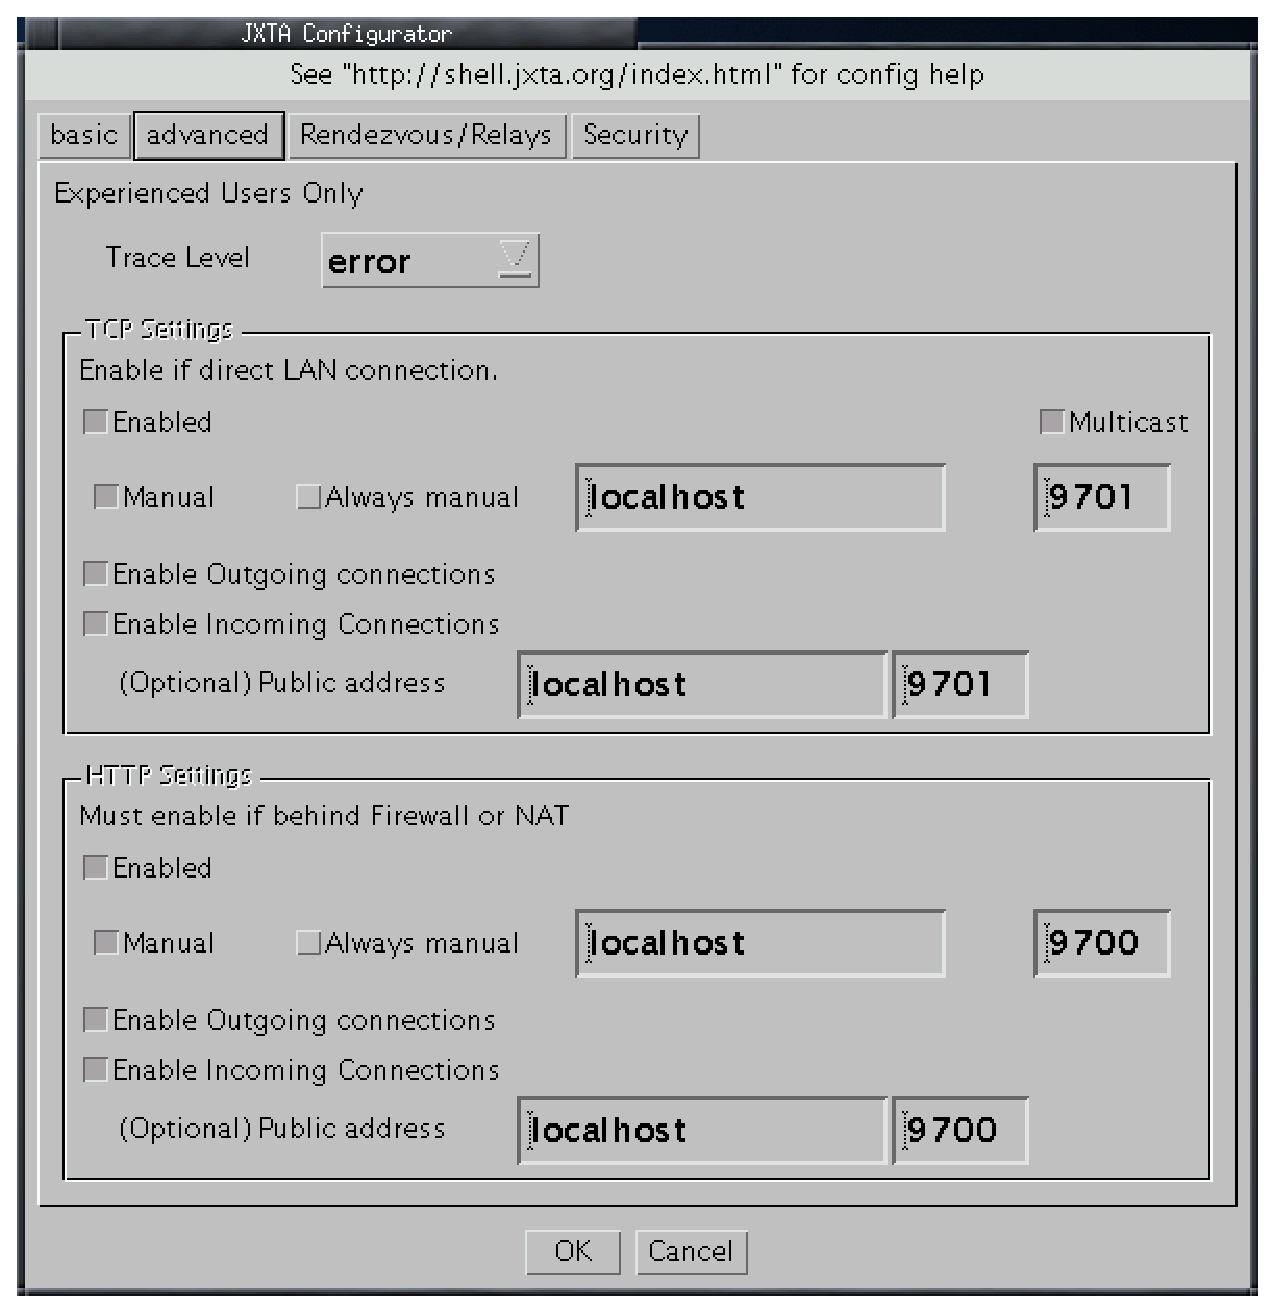
\includegraphics{fig/JXTAConfig.ps}}
  \label{fig:platform}
  \caption{General architecture of DIET/JXTA}
 \end{center}
\end{figure}

\item{\textbf{Second step}: registering a SeD to the MA. The same
    paths must be set:\\ (\texttt{<DIET\_root>/src/SeD/.libs} for
    \texttt{LD\_LIBRARY\_PATH}.) Be sure that the \texttt{parentName}
    inside the configuration file matches the name
    of the MA$_{DIET}$ previously launched. The command to run is:\\\\
    \texttt{\$ java -cp <JXTA\_LIBS> JXTASeD
      <DIET\_SeD\_config\_file>\linebreak[4] <computation\_abilities>}
    \\\\ If you want to put LA(s) between the MA and the
    SeD, launch the following command before loading the SeD:\\\\
    \texttt{\$ java LA <DIET\_LA\_config\_file>}\\\\ Check the DIET
    tree coherence and the \texttt{parentName} variables inside the
    configuration files. }

\item{\textbf{Third step}: Launch a JXTA client with the command:\\\\
                    \texttt{\$ java -cp <JXTA\_LIBS> ClientJXTA <pb>}}

\end{itemize}

At this point, you still haven't tested the Multi-MA. To achieve this,
launch other MA$_{JXTA}$(s) and launch again the client.

Scripts have been left at your disposal. You just need to check the
environment variables and paths required. As said before, only one
JXTA peer can be run in one directory, so each script is inside a
different one. These directories have to be edited (for configuration), are named
\texttt{MMA1/}, \texttt{MMA2/}, \texttt{MMA3/}, \texttt{LA1/},
\texttt{SeD1/}, \texttt{SeD2/} and \texttt{client/}.  and are located
in : \texttt{<DIET\_root>/src/example/jxta/scripts}.
 



%
% JuxMem extension
%
\newpage
%****************************************************************************%
%* DIET User's Manual JuxMem use chapter file                               *%
%*                                                                          *%
%*  Author(s):                                                              *%
%*    - Mathieu Jan (Mathieu.Jan@irisa.fr)                                  *%
%*                                                                          *%
%* $LICENSE$                                                                *%
%****************************************************************************%

\chapter{JuxMem extension}
\label{ch:juxmem}

\section{Introduction}

With the release of version 2.0 of the DIET toolkit, we introduce the
ability to use JuxMem for managing persistent data blocks. This
section shortly describes how to use JuxMem inside DIET, as it is an
on going work.

\section{Overview of JuxMem}

JuxMem, stands for Juxtaposed Memory, implements the concept of data
sharing service for grid, based on a compromise between DSM systems
and P2P systems. JuxMem decouples data management from grid
computation, by providing location transparency as well as data
persistence in a dynamic environnement. JuxMem is based on the P2P
platform called JXTA, which stands for Juxtaposed. For more
information about JuxMem, please check the available documentation on
the web site of JuxMem~\cite{JuxMem}.

\section{How to configure DIET to use JuxMem?}

DIET currently needs JuxMem version 0.2 to work. This version can be
downloaded on the web site of JuxMem~\cite{JuxMem}. For configuring
and building JuxMem, please check the README file included in this
0.2 release of JuxMem. When the \texttt{--enable-JuxMem} option is
activated, you need to have JuxMem-C build, so please read the
documentation for building JuxMem-C. Currently, for configuring DIET
in order to use JuxMem you need to specify the build path of JuxMem,
JXTA-C and APR using respectively the \texttt{--with-juxmem},
\texttt{--with-jxta-c} and \texttt{--with-apr} options.
Note that APR (Apache Portable Runtime) is a requirement of both
JuxMem-C and JXTA-C.

When DIET is configured to use JuxMem, SeDs are able to store data
blocks inside JuxMem. Please be carefull as it does not mean that you
have a JuxMem platform deployed and usable!  In a first step, you must
deploy a JuxMem platform as described in the documentations of
JuxMem. This JuxMem platform is currently based on JuxMem-J2SE,
JuxMem-C is only used to play the role of a JuxMem client within a
DIET SeD. Please read the README file of JuxMem to build and deployed
a JuxMem platform.

\section{Example}

A simple example of the JuxMem usage inside DIET can be found in the
dmat\_manips sample. The name of the client is
\texttt{clientJuxMem}. This example stores DIET matrices inside JuxMem, 
and allows next computations to retrieve these matrices directly from
JuxMem. Clients therefore avoid unnecessary tranfers of matrices as
they only need to transfer the ID of the data returned by JuxMem. More
documentation and examples will be available in the future.

\section{Troubleshooting}

If you encounter any problem, you can try get help from the
JuxMem-discuss mailing list
\url{<juxmem-discuss@lists.gforge.inria.fr>}. Do not forget to include
in your e-mails the exact error message, your hardware description,
your OS name and version, and the JuxMem version number.  However,
please do understand that this is an on going work and therefore no
full support is provided.


%%%%
% BIBLIO
%%%%

\bibliographystyle{plain}
\bibliography{UsersManual}

\end{document}
